%%%%%%%%%%%%%%%%%%%%%%%%%%%%%%%%%%%%%%%%%%%%%%%%%%%%%%%%%%%%%%%%%%%
%                                                                 %
%  GEANT manual in LaTeX form                                     %
%                                                                 %
%  Version 1.00                                                   %
%                                                                 %
%  Last Mod. 8 June 1993  17:20  MG                               %
%                                                                 %
%%%%%%%%%%%%%%%%%%%%%%%%%%%%%%%%%%%%%%%%%%%%%%%%%%%%%%%%%%%%%%%%%%%
\documentstyle[11pt,fleqn,epsfig,crngeant,bibunits,fontcmds,multicol]{cernman}
\newcommand{\Title}{GEANT User's Guide}%           Title for document
\psfigdriver{DVIPS}
\makeindex
\romanfont{times}
\PScommands% Initialize PS boxes
\newmathalphabet*{\mathtt}{cmtt}{m}{n}
\newmathalphabet*{\mathbf}{cmr}{b}{n}
\begin{document}
%  ==================== Front material ============================
%%%%%%%%%%%%%%%%%%%%%%%%%%%%%%%%%%%%%%%%%%%%%%%%%%%%%%%%%%%%%%%%%%%
%                                                                 %
%   GEANT -- Short write ups -- LaTeX Source                      %
%                                                                 %
%   Front Material: Title page,                                   %
%                   Copyright Notice                              %
%                   Preliminary Remarks                           %
%                   Table of Contents                             %
%   EPS file      : cern15.eps, cnastit.eps                       %
%                                                                 %
%   Editor: Michel Goossens / CN-AS                               %
%   Last Mod.: 11 June 1993 10:30 mg                              %
%                                                                 %
%%%%%%%%%%%%%%%%%%%%%%%%%%%%%%%%%%%%%%%%%%%%%%%%%%%%%%%%%%%%%%%%%%%
 
%%%%%%%%%%%%%%%%%%%%%%%%%%%%%%%%%%%%%%%%%%%%%%%%%%%%%%%%%%%%%%%%%%%%
%    Tile page                                                     %
%%%%%%%%%%%%%%%%%%%%%%%%%%%%%%%%%%%%%%%%%%%%%%%%%%%%%%%%%%%%%%%%%%%%
\latex{\def\Ptitle#1{\special{ps: /Printstring (#1) def}
                       \epsfbox{eps/cnastit.eps}}}
 
\begin{titlepage}
%begin{latexonly}
\vspace*{-23mm}%

\includegraphics[height=30mm]{cern.eps}
\hfill
\raise8mm\hbox{\Large\bf CERN Program Library Long Writeup W5013}
\hfill\mbox{}
\begin{center}
\mbox{}\\[6mm]
\mbox{\Ptitle{GEANT}}\\[3cm]
{\Huge Detector Description and}\\[2cm]
{\Huge Simulation Tool}\\[4cm]
{\Large Application Software Group}\\[6mm]
{\Large Computing and Networks Division}\\[2cm]
\end{center}
\vfill
\begin{center}\Large CERN Geneva, Switzerland\end{center}
%end{latexonly}
\begin{htmlonly}
\begin{center}
\Large CERN Program Library Long Writeup W5013\\[1cm]
\Huge GEANT\\[2cm]
\Large Detector Description and Simulation Tool\\[1cm]
\large IT/ASD Group\\
\large CERN, Geneva, Switzerland
\end{center}
\end{htmlonly}
\end{titlepage}

%%%%%%%%%%%%%%%%%%%%%%%%%%%%%%%%%%%%%%%%%%%%%%%%%%%%%%%%%%%%%%%%%%%%
%    Copyright  page                                               %
%%%%%%%%%%%%%%%%%%%%%%%%%%%%%%%%%%%%%%%%%%%%%%%%%%%%%%%%%%%%%%%%%%%%

\thispagestyle{empty}
\framebox[\textwidth][t]{\hfill\begin{minipage}{0.96\textwidth}%
\vspace*{3mm}
\begin{center}Copyright Notice\end{center}
\parskip\baselineskip

\textbf{GEANT -- Detector Description and Simulation Tool}
 
\copyright{} Copyright CERN, Geneva 1993
 
Copyright and any other appropriate legal protection of these
computer programs and associated documentation reserved in all
countries of the world.
 
These programs or documentation may not be reproduced by any
method without prior written consent of the Director-General
of CERN or his delegate.
 
Permission for the usage of any programs described herein is
granted apriori to those scientific institutes associated with
the CERN experimental program or with whom CERN has concluded
a scientific collaboration agreement.
 
CERN welcomes comments concerning the Geant code
but undertakes no obligation for the maintenance of the programs,
nor responsibility for their correctness, and accepts no liability
whatsoever resulting from the use of its programs.
 
Requests for information should be addressed to:
\vspace*{-.5\baselineskip}
\begin{center}\ttfamily
\begin{tabular}{l}
CERN Program Library Office              \\
CERN-IT Division                         \\
CH-1211 Geneva 23                        \\
Switzerland                              \\
Tel.      +41 22 767 4951                \\
Fax.      +41 22 767 7155                \\
Email:    cernlib@cern.ch                \\
WWW:      http://wwwinfo.cern.ch/asd/index.html
\end{tabular}
\end{center}
\vspace*{2mm}
\end{minipage}\hfill}%end of minipage in framebox
\vspace{6mm}
 
{\bf Trademark notice: All trademarks appearing in this guide are acknowledged as such.}
\vfill

\begin{tabular}{l@{\quad}l@{\quad}>{\small\ttfamily}l}
\emph{Contact Persons}:       & IT/ASD/SImulation section & (giani\atsign cern.ch)\\[1mm]
\emph{Documentation Consultant}: & Michel Goossens /IT    & (goossens\atsign cern.ch)\\[1cm]
\textem{Edition -- March 1994}
\end{tabular}
\newpage
 

%  ==================== Body of text ==============================
\pagenumbering{arabic}
\setcounter{page}{1}
 
%%%%%%   Catalog of Program packages and entries%%%%
 
\def\Rtnr{Catalog}%Dummy routine name to appear at bottom of page
%%%%%%%%%%%%%%%%%%%%%%%%%%%%%%%%%%%%%%%%%%%%%%%%%%%%%%%%%%%%%%%%%%%
%                                                                 %
%  GEANT manual in LaTeX form   	                          %
%                                                                 %
%  Michel Goossens (for translation into LaTeX)                   %
%  Version 2.00                                                   %
%  Last Mod.  2 Jun 1998  17:10   MG                              %
%                                                                 %
%%%%%%%%%%%%%%%%%%%%%%%%%%%%%%%%%%%%%%%%%%%%%%%%%%%%%%%%%%%%%%%%%%%
%%% Generated from headings
\chapter{Catalog of Geant sections}
\begin{DLtt}{12345678}
\item[AAAA001] Foreword
\item[AAAA002] Introduction to the manual
\item[BASE001] Introduction to GEANT
\item[BASE010] Simplified Program Flow Chart
\item[BASE020] The data structures and their relationship
\item[BASE040] Summary of Data Records
\item[BASE090] The reference systems and physical units
\item[BASE100] Examples of GEANT application
\item[BASE110] The system initialisation routines
\item[BASE200] Steering routines for event processing
\item[BASE280] Storing and retrieving JRUNG and JHEAD information
\item[BASE299] The banks JRUNG and JHEAD
\item[BASE300] Example of user termination routine
\item[BASE400] Debugging facilities
\item[BASE410] Utility Routines
\item[BASE420] The random number generator
\item[CONS001] Introduction to the section CONS
\item[CONS100] Material definition
\item[CONS101] Retrieve material cross-sections and stopping power
\item[CONS110] Mixtures and Compounds
\item[CONS199] The Material data structure JMATE
\item[CONS200] Tracking medium parameters
\item[CONS210] Special Tracking Parameters
\item[CONS300] Particle definition
\item[CONS310] Branching Ratios and Particle Decay Modes
\item[DRAW001] Introduction to the Drawing package
\item[DRAW010] The Ray-tracing package
\item[DRAW110] Drawing a Volume -- Case 1
\item[DRAW115] Drawing a Volume Projection view -- Case 2
\item[DRAW120] Draw a volume cut view
\item[DRAW130] Draw Particle Trajectories
\item[DRAW140] Drawing Track Hits in Sensitive Detectors
\item[DRAW210] Drawing the geometrical tree
\item[DRAW220] Drawing volume specifications
\item[DRAW300] Handling View banks
\item[DRAW399] The data structure JDRAW
\item[DRAW400] Utility routines of the drawing package
\item[GEOM001] The geometry package
\item[GEOM010] Tracking inside volumes and optimisation
\item[GEOM020] ``MANY'' Volumes and boolean operations on volumes
\item[GEOM050] The GEANT shapes
\item[GEOM100] Creation of a volume
\item[GEOM110] Positioning a volume inside its mother
\item[GEOM120] Positioning a volume inside its mother with parameters
\item[GEOM130] Division of a volume into a given number of cells
\item[GEOM140] Division of a Volume into cells of a given size
\item[GEOM150] Division of a volume - general case
\item[GEOM199] The volume data structure -- JVOLUM
\item[GEOM200] Rotation matrices
\item[GEOM299] The rotation matrix data structure JROTM
\item[GEOM300] Finding in which volume a point is
\item[GEOM310] Finding distance to next boundary
\item[GEOM320] Reference system transformations
\item[GEOM400] Pseudo-division of a volume
\item[GEOM410] Ordering the contents of a volume
\item[GEOM500] Volume attributes
\item[GEOM600] User initialisation of the common block /GCVOLU/
\item[GEOM700] Medium search statistics
\item[GEOM900] End of geometry definition
\item[GEOM910] The CADINT Interface
\item[HITS001] The detector response package
\item[HITS100] Sensitive DETector definition
\item[HITS105] Detector aliases
\item[HITS110] DETector hit parameters
\item[HITS120] DETector Digitisation parameters
\item[HITS130] User detector parameters
\item[HITS199] The SET data structure JSET
\item[HITS200] Routines to store and retrieve HITS
\item[HITS299] The JHITS data structure
\item[HITS300] Routines to store and retrieve DIGItisations
\item[HITS399] The JDIGI data structure
\item[HITS400] Intersection of a track with a cylinder or a plane
\item[HITS500] Digitisation for drift- or MWP- Chambers
\item[HITS510] Digitisation for drift chambers
\item[IOPA001] The I/O routines
\item[IOPA200] ZEBRA sequential files handling
\item[IOPA300] Data structure I/O with sequential files
\item[IOPA400] ZEBRA direct access files handling
\item[IOPA500] Data structure I/O with direct access files
\item[KINE001] Section KINE
\item[KINE100] Storing and retrieving vertex and track parameters
\item[KINE199] The data structures JVERTX and JKINE
\item[KINE200] Interface to the Lund Monte Carlo
\item[KINE210] $\tau ^{\pm }$ generation and decay
\item[PHYS001] Introduction to the section PHYS
\item[PHYS010] Compute the occurrence of a process
\item[PHYS100] Steering routine for physics initialisation
\item[PHYS210] Total cross-section for e+e- pair production by photons
\item[PHYS211] Simulation of e-e+ pair production by photons
\item[PHYS220] Total cross-section for Compton scattering
\item[PHYS221] Simulation of Compton scattering
\item[PHYS230] Total cross-section for photoelectric effect
\item[PHYS231] Simulation of photoelectric Effect
\item[PHYS240] Photon-induced fission on heavy materials
\item[PHYS250] Total cross-section for Rayleigh scattering
\item[PHYS251] Simulation of Rayleigh scattering
\item[PHYS260] \v{C}erenkov photons
\item[PHYS320] Gaussian multiple scattering
\item[PHYS325] Moli\`ere scattering
\item[PHYS328] Plural scattering
\item[PHYS330] Ionisation processes induced by e+/e-
\item[PHYS331] Simulation of the delta-ray production
\item[PHYS332] Simulation of energy loss straggling
\item[PHYS333] Information about energy loss fluctuations
\item[PHYS334] Models for energy loss fluctuations in thin layers
\item[PHYS337] Birks' saturation law
\item[PHYS340] Total cross-section and energy loss for bremsstrahlung by e-e+
\item[PHYS341] Simulation of discrete bremsstrahlung by electrons
\item[PHYS350] Total cross-section for e+e- annihilation
\item[PHYS351] Simulation of e+e- annihilation
\item[PHYS360] Synchrotron radiation
\item[PHYS400] Simulation of particle decays in flight
\item[PHYS410] Rotations and Lorentz transformation
\item[PHYS430] Ionisation processes for muons and protons
\item[PHYS431] Ionisation processes for heavy ions
\item[PHYS440] Total cross-section and energy loss for bremsstrahlung by Muons
\item[PHYS441] Simulation of discrete bremsstrahlung by muons
\item[PHYS450] Total cross-section and energy loss for e-e+ pair production by muons
\item[PHYS451] Simulation of e+e- pair production by muons
\item[PHYS460] Muon-nucleus interactions
\item[PHYS510] The GEANT/GHEISHA Interface
\item[PHYS520] The GEANT/FLUKA Interface
\item[PHYS530] The GEANT/MICAP interface
\item[TRAK001] The tracking package
\item[TRAK110] Steering routine to track one event
\item[TRAK120] Steering routine to track one particle
\item[TRAK130] Tracking one particle through a volume
\item[TRAK200] The tracking routines block diagrams
\item[TRAK300] Storing secondary tracks in the stack
\item[TRAK310] Altering the order of tracking secondary particles
\item[TRAK399] The temporary stack data structure JSTAK
\item[TRAK400] Handling of track space points
\item[TRAK499] The space point data structure JXYZ
\item[TRAK500] Tracking routines in magnetic field
\item[XINT001] The interactive version of GEANT
\item[XINT002] Introduction to the Interactive version of GEANT
\item[XINT010] Screen views of GEANT++
\item[ZZZZ010] List of COMMON Blocks
\item[ZZZZ999] Index of Documented GEANT routines
\end{DLtt}

 
\let\LARGE\large
\let\Large\large
\let\DL\DLtt 

% Here come the different files to be included
 
%%     XINT part     %%
 
\begin{bibunit}[unsrt]
\renewcommand{\bibname}{XINT Bibliography}
\cleardoublepage
%%%%%%%%%%%%%%%%%%%%%%%%%%%%%%%%%%%%%%%%%%%%%%%%%%%%%%%%%%%%%%%%%%%
%                                                                 %
%  GEANT manual in LaTeX form                              %
%                                                                 %
%  Michel Goossens (for translation into LaTeX)                   %
%  Version 1.00                                                   %
%  Last Mod. Jan 24 1991  1300   MG + IB                          %
%                                                                 %
%%%%%%%%%%%%%%%%%%%%%%%%%%%%%%%%%%%%%%%%%%%%%%%%%%%%%%%%%%%%%%%%%%%
\Documentation{R.Brun}
\Submitted{15.06.84}   \Revised{19.12.93}
\Version{Geant 3.16}    \Routid{XINT001}
\Makehead{The interactive version of GEANT}
 
The interactive version is an essential tool for users who are
in charge of the design of a detector.
In addition to all the batch tools which are also available, the
interactive user can call one by one and in any order all the basic
functions of {\tt GEANT} to:
\begin{itemize}
\item design or modify the geometry of the setup;
\item exploit the drawing package in a more efficient way;
\item change the running conditions on a event by event basis.
\end{itemize}
The system is based on the {\tt KUIP}~\cite{bib-KUIP}
command processor.
The user has to know a minimum about {\tt KUIP} and should read
at least the first chapter of the manual.

A set of encapsulated Postscript files have been collected in
a new section XINT010. They illustrate the visualization possibilities
of the interactive version of {\tt GEANT}. 

\section{Invoking the interactive version}
Instead of writing a MAIN program to initialize the Geant batch
version, it is possible to use the MAIN interactive program (GXINT321.F)
provided in /cern/pro/lib exactly as the library LIBGEANT321.A. The user
has simply to insert in his link file the file GXINT321.F as the main
program, followed by the user object code and by the library LIBGEANT321.A.
\\[.5em] Example: \\[.1em]
       PROGRAM GXINT \\[.1em]
* \\[.1em]
*     GEANT main program. To link with the MOTIF user interface \\[.1em]
*     the routine GPAWPP(NWGEAN,NWPAW) should be called, whereas \\[.1em]
*     the routine GPAW(NWGEAN,NWPAW) gives access to the basic \\[.1em]
*     graphics version. \\[.1em]
* \\[.1em]
      PARAMETER (NWGEAN=3000000,NWPAW=1000000) \\[.1em]
      COMMON/GCBANK/GEANT(NWGEAN) \\[.1em]
      COMMON/PAWC/PAW(NWPAW) \\[.1em]
* \\[.1em]
      CALL GPAWPP(NWGEAN,NWPAW) \\[.1em]
* \\[.1em]
      END \\[.5em]
The user has to set the desired value of NWGEAN and NWPAW for the
GEANT and PAW Zebra stores, and to call the desired initialization routine:
\begin{itemize}
\item GPAW to initialize, besides GEANT, also HIGZ and to include the full
      functionality of PAW;
\item GPAWPP to initialize, besides GEANT and HIGZ, also the Motif version 
      and to include the full functionality of Paw++;
\item USER initialization routine, to do anything else (for example a UGINIT-
      like routine or a gxint315.f--like routine). 
\end{itemize}
The interactive version, after the initialization, gives the control to the
user at the prompt GEANT $>$ ; then it is possible to type and execute 
commands (corresponding to batch routines) to edit the geometry, the materials
or the tracking media at run time. It is also possible to execute commands
to visualize the detectors, to set the kinematics and to run events. Again
interactively, one can spy the histograms, change the kinematics, and run
more events (visualizing the tracks and the hits, for example). The GXINT
chapter contains in the following pages a full description of the available
GEANT commands. See the PAW, KUIP, DZDOC, HIGZ manuals for a description of
the relative commands executable from GEANT. All the commands are also
documented by an on-line help. (Try to type HELP at the first GEANT $>$ prompt).
In the interactive version, a COMIS interface is also available: COMIS is a
FORTRAN interpreter which allows:
\begin{itemize}
\item to edit at run time important routines like UGEOM, GUSTEP, GUKINE, etc.
\item to `execute' them from the interactive session, without having to 
      recompile and relink, by typing commands like CALL UGEOM.F.
\end{itemize}
Of course the interpreter is slower than the compiled object code,
then, since GEANT321, it is also possible to invoke the native compiler and
to link dinamically to the executable the compiled routine (see the COMIS 
manual for further details).


The following write ups describe individual commands which can be typed
one by one at the terminal, or grouped into macros which can be edited
and saved in the {\tt KUIP} environment.

The commands are listed in subsection 1 - 13:

\begin{center}\begin{tabular}{ll}
1. &  General GEANT \\
2. & Clipping commands GEANT/CVOL \\
3. & Drawing commands GEANT/DRAWING \\
4. & Graphics control commands GEANT/DRAWING \\
5. & Geometry commands GEANT/GEOMETRY \\
6. & Volume creation commands GEANT/CREATE \\
7. & Control commands GEANT/CONTROL \\
8. & ZEBRA/RZ commands GEANT/RZ \\
9. & ZEBRA/FZ commands GEANT/FZ \\
10. & Data structure commands GEANT/DZ \\
11. & Scanning commands GEANT/SCAN \\
12. & Physics parameter commands GEANT/PHYSICS \\
13. & List commands GEANT/LISTS \\
\end{tabular}\end{center}

\section{The Motif Interface}
The interactive version 3.21 contains an object oriented Motif-based user
interface. It can be accessed specifying `m' as workstation type.
The full functionality of the X11 version remains available, while new 
Motif-specific features have been added. \\[1em]
\section{The main ideas} 
The {\tt GEANT} data structures are 
considered as KUIP browsable classes and their
contents as `objects' on which one can perform actions 
(the {\tt GEANT} commands).
According to the Motif conventions, an object can be selected clicking the
left button of the mouse (when the cursor is on the icon representing that
object). Clicking then on the right button of the mouse, a menu of possible
commands will appear (double clicking on the left button the first action of
this list will be executed); 
the selected command will perform the relative actions
on the selected object. Such actions (like drawing, for example) can be
executed either directly or via the use of an automatically opened Motif panel.
Objects drawn in the graphics window can be `picked' as well (for example,
volumes, tracks, hits); clicking the right button when the cursor is on the
selected object, a menu of possible actions on that object is displayed.
Users can finally define Motif panels containing buttons corresponding to the
most frequently used commands. An on-line help is available for any specific
subject. \\[1em]

\section {The Geant++ Executive Window}
It replaces the normal dialog window; it contains a Transcript Pad, where the
text output of the executed commands is displayed, and an Input Pad, where the
user can still type the desired commands in the old style. \\[1em]
The {\tt Geant++} Main File Browser \\[1em]
On the left side it displays a list of the {\tt GEANT} data structures, of the 
available commands, file, macros and Zebra divisions used. Selecting one of
them, the full list of icons representing the objects of that class is shown
in the main area of the browser. Proceeding as described before, it is 
possible to perform actions on the classes (like create a new object) or on
the objects belonging to them. It is possible to create menus of commands
just clicking on the string `commands' at the top line of the browser. \\[1em]
The Geant++ Graphics Window \\[1em]
Any object to be drawn in the graphics window can be stored in the current
picture file (automatically opened after each NEXT command) via a call to 
IGPID (see Higz manual). It can be afterwards `picked' as described before.
In the case of commands executed via the use of Motif panels, some input values
can be set with a slider ranging in the specifed range for the relative
variable; moving the slider (after having clicked on the right-hand `activating
box') the relative action is performed in the graphics
window when releasing the button of the mouse; when in `drag mode', the 
action is performed {\it while} moving the slider (keeping the left button
pressed): especially when double buffering has been selected, this can be
useful for real time manipulations.\\[1em]
\section {An Example}
Start your {\tt GEANT321} executable module 
(linked with GXINT321 and Motif1.2);
\\[.5em] type `m' as workstation type;
\\[.5em] click the left button of the mouse after positioning the cursor on the 
string VOLU in the browser;
\\[.5em] click the left button of the mouse after positioning the cursor on 
any icon in the main area of the browser;
\\[.5em] click now the right button of the mouse and keep it pressed;
\\[.5em] move the mouse to select the action `Tree' and release the button;
\\[.5em] the drawing of the logical tree will be displayed in the graphics
window;
\\[.5em] position the cursor on the drawing of a box (containing a volume name)
in the graphics window, click the right button and keep it pressed;
\\[.5em] release the button selecting the action `Dspec';
\\[.5em] the command DSPEC for that volume will be executed in a separate
window;
\\[.5em] repeat the exercise selecting this time the action `Dspe3d';
\\[.5em] the DSPEC will be executed in the first window, the volume 
specifications will be printed in a separate window and a Motif panel will
appear;
\\[.5em] click the left button of the mouse positioning the cursor in the Motif
panel on the `Value changed' button, and select the DRAG option;
\\[.5em] click now the left button on the `activating box' on the right of
the `Theta' slider;
\\[.5em] click on the `Theta' slider and, keeping pressed the left button of the
mouse, move it right-wards;
\\[.5em] the drawing in the graphics window will rotate;
\\[.5em] release the button and type `igset 2buf 1' in the executive window;
\\[.5em] restart moving the slider as before. 

	%%%%%%%%%%%%%%%%%%%%%%%%%%%%%%%%%%%%%%%%%%%%%%%%%%%%%%%%%%%%%%%%%%%
%                                                                 %
%  GEANT manual in LaTeX form                                     %
%                                                                 %
%  Version 1.00                                                   %
%                                                                 %
%  Last Mod. 15 June 1993 19:00  MG                               %
%                                                                 %
%%%%%%%%%%%%%%%%%%%%%%%%%%%%%%%%%%%%%%%%%%%%%%%%%%%%%%%%%%%%%%%%%%%
\Authors{S.Giani}     \Origin{Same}
\Submitted{15.06.84}   \Revised{20.03.94}
\Version{Geant 3.21}\Routid{XINT002}
\Makehead{Introduction to the Interactive version of GEANT}

\newif\ifMENUtext \MENUtexttrue
\newcommand{\DEFMENU}[3]{% {level}{name}{path}
\section{#3}}

\newcommand{\INDEX}[1]{% protect underscores
{\def\_{\char'137}\index{#1@{\tt #1}}}}

\newcommand{\DEFCMD}[5]{% {menulabel}{cmdlabel}{menupath}{cmdname}{args}
\par%\begin{minipage}{\textwidth}
\subsection{#4 #5 \label{#1:#2}\INDEX{#3/#4}\INDEX{#4}}}
\newcommand{\ENDCMD}{\par}%\end{minipage}\par}

\newcommand{\DEFCBIG}[5]{% DEFCMD with long guidance text
\subsection{#4 #5 \label{#1:#2}\INDEX{#3/#4}\INDEX{#4}}}
\newcommand{\ENDCBIG}{\par}

\newcommand{\BEGARG}{%
\par\begin{longtable}{lcp{.75\textwidth}}\endhead}
\newcommand{\DEFARG}[4]{% {parname}{partype}{prompt}{default}
{\tt #1} & #2 & ``#3'' {\tt #4} \\}
\newcommand{\ENDARG}{%
\end{longtable}\par}

\newcommand{\BEGOPT}[1]{% {parname}
\par\noindent Possible {\tt #1} values are:
\par\noindent \begin{tabular}{lp{.85\textwidth}}}
\newcommand{\DEFOPT}[2]{% {option}{text}
{\tt #1} & #2 \\[1ex]}
\newcommand{\ENDOPT}{\end{tabular}\par}

\newcommand{\BEGTEXT}{\par}
\newcommand{\ENDTEXT}{}
\newcommand{\ENDVERB}{\par}
\newcommand{\EMPTY}{{\tt '\char`\ '}}% empty string
\newcommand{\BRA}{$\langle$}% left angle <
\newcommand{\KET}{$\rangle$}% right angle >
\newcommand{\PIPE}{$|$}% vertical bar |
\newcommand{\DQUOTE}{{\tt "}}% double quote "

%\begin{document}
\DEFMENU{0}{GEANT}{GEANT}
\ifMENUtext
   \par
GEANT specific commands.  


\fi
\DEFMENU{1}{CVOL}{GEANT/CVOL}
\ifMENUtext
   \par
Clipping commands.  The hidden line removal technique is necessary to 
   visualize properly very complex detectors. At the same time, it can be 
   useful to visualize the inner elements of a detector in detail. For this 
   purpose, the commands menu CVOL has been developed: these commands allow 
   subtractions (via boolean operation) of given shapes from any part of the 
   detector, therefore showing its inner contents. It is possible to clip each 
   different volume by means of a different shape (BOX , TUBE, CONE, SPHE are 
   available). If '*' is given as the name of the volume to be clipped, all 
   volumes are clipped by the given shape.  A volume can be clipped at most 
   twice (even by different shapes); if a volume is explicitely clipped twice, 
   the '*' will not act on it anymore. Giving '.' as the name of the volume to 
   be clipped will reset the clipping.  


\fi

\DEFCMD{GC}{BOX}{GEANT/CVOL}{BOX}{ cnnv [ xmin xmax ymin ymax zmin zmax ]}

\BEGARG
\DEFARG{CNNV}{C}{ Name of volume to be clipped          }{ D='*   '}
\DEFARG{XMIN}{R}{ Lower limit of the Shape X coordinate }{ D=-10000.}
\DEFARG{XMAX}{R}{ Upper limit of the Shape X coordinate }{ D=-9999.}
\DEFARG{YMIN}{R}{ Lower limit of the Shape Y coordinate }{ D=-10000.}
\DEFARG{YMAX}{R}{ Upper limit of the Shape Y coordinate }{ D=-9999.}
\DEFARG{ZMIN}{R}{ Lower limit of the Shape Z coordinate }{ D=-10000.}
\DEFARG{ZMAX}{R}{ Upper limit of the Shape Z coordinate }{ D=-9999.}
\ENDARG

   \par
This command performs a boolean subtraction between the volume CNVV and a 
   box placed in the MARS according the values of the given coordinates. See 
   also CVOL.  The following commands will clip by a box, with a vertex at the 
   origin, the volume specified by NAME (a valid string for the NAME of the 
   volume can be found using the DTREE command).  
\begin{verbatim}
    EXAMPLE -
    dopt hide on
    satt * seen -2
    draw NAME 40 40 0 10 10 .01 .01
    next
    box NAME 0 1000 0 1000 0 1000
    draw NAME 40 40 0 10 10 .01 .01
    box .
\end{verbatim}

\ENDCMD

\DEFCMD{GC}{TUBE}{GEANT/CVOL}{TUBE}{ cnvv [ rmax zdem xmed ymed zmed ]}

\BEGARG
\DEFARG{CNVV}{C}{ Name of volume to be clipped          }{ D='*   '}
\DEFARG{RMAX}{R}{ External radius of tube               }{ D=0.1}
\DEFARG{ZDEM}{R}{ Half length of tube axis              }{ D=0.1}
\DEFARG{XMED}{R}{ Center X coordinate                   }{ D=-10000.}
\DEFARG{YMED}{R}{ Center Y coordinate                   }{ D=-10000.}
\DEFARG{ZMED}{R}{ Center Z coordinate                   }{ D=-10000.}
\ENDARG

   \par
This command performs a boolean subtraction between the volume CNVV and a 
   tube; the tube has the given parameters and is placed in the MARS according 
   the given coordinates of its center.  See also CVOL.  The following 
   commands will clip, by a tube, positioned according to the given 
   parameters, the volume specified by NAME (a valid string for the NAME of 
   the volume can be found using the DTREE command).  
\begin{verbatim}
    EXAMPLE -
    dopt hide on
    satt * seen -2
    draw NAME 40 40 0 10 10 .01 .01
    next
    tube * 500 1000 500 0 0
    draw NAME 40 40 0 10 10 .01 .01
    box .
\end{verbatim}

\ENDCMD

\DEFCMD{GC}{CONE}{GEANT/CVOL}{CONE}{ cnvv [ rmax1 rmax2 zdem xmed ymed zmed ]}

\BEGARG
\DEFARG{CNVV}{C}{ Name of volume to be clipped          }{ D='*   '}
\DEFARG{RMAX1}{R}{ Min external radius                   }{ D=0.1}
\DEFARG{RMAX2}{R}{ Max external radius                   }{ D=0.1}
\DEFARG{ZDEM}{R}{ Half length of cone axis              }{ D=0.1}
\DEFARG{XMED}{R}{ Center X coordinate                   }{ D=-10000.}
\DEFARG{YMED}{R}{ Center Y coordinate                   }{ D=-10000.}
\DEFARG{ZMED}{R}{ Center Z coordinate                   }{ D=-10000.}
\ENDARG

   \par
This command performs a boolean subtraction between the volume CNVV and a 
   cone; the cone has the given parameters and is placed in the MARS according 
   to the given coordinates of its center.  See also CVOL.  The following 
   commands will clip by a cone, positioned according the given parameters, 
   the volume specified by NAME (a valid string for the NAME of the volume can 
   be found using the DTREE command).  
\begin{verbatim}
    EXAMPLE -
    dopt hide on
    satt * seen -2
    draw NAME 40 40 0 10 10 .01 .01
    next
    cone * 1 750 1000 0 0 1000
    draw NAME 40 40 0 10 10 .01 .01
    box .
\end{verbatim}

\ENDCMD

\DEFCMD{GC}{SPHE}{GEANT/CVOL}{SPHE}{ cnvv [ rmax xmed ymed zmed ]}

\BEGARG
\DEFARG{CNVV}{C}{ Name of volume to be clipped          }{ D='*   '}
\DEFARG{RMAX}{R}{ External radius of sphere             }{ D=0.1}
\DEFARG{XMED}{R}{ Center X coordinate                   }{ D=-10000.}
\DEFARG{YMED}{R}{ Center Y coordinate                   }{ D=-10000.}
\DEFARG{ZMED}{R}{ Center Z coordinate                   }{ D=-10000.}
\ENDARG

   \par
This command performs a boolean subtraction between the volume CNVV and a 
   sphere; the sphere has the given parameters and is placed in the MARS 
   according to the given coordinates of its center.  See also CVOL. The 
   following commands clip by a sphere, positioned according to the given 
   parameters, the volume specified by NAME (a valid string for the NAME of 
   the volume can be found using the DTREE command).  EXAMPLE - 
\begin{verbatim}
    dopt hide on
    satt * seen -2
    draw NAME 40 40 0 10 10 .01 .01
    next
    sphe * 500 0 0 500
    draw NAME 40 40 0 10 10 .01 .01
    box .
\end{verbatim}

\ENDCMD

\DEFCMD{GC}{VALCUT}{GEANT/CVOL}{VALCUT}{ xcut ycut zcut}

\BEGARG
\DEFARG{XCUT}{R}{x coordinate of cutted value}{ D=0.}
\DEFARG{YCUT}{R}{y coordinate of cutted value}{ D=0.}
\DEFARG{ZCUT}{R}{z coordinate of cutted value}{ D=0.}
\ENDARG

   \par
It allows the cutting in the ray-tracing. All the volumes are cutted from 
   XCUT to +BIG along the x axis, from YCUT to +BIG along the y axis and from 
   ZCUT to +BIG along the z axis.  

\ENDCMD
\newpage
\DEFMENU{1}{DRAWING}{GEANT/DRAWING}
\ifMENUtext
   \par
Drawing commands. These commands allow the visualization in several ways of 
   the volumes defined in the geometrical data structure. It is possible to 
   draw the logical tree of volumes belonging to the detector (DTREE), to show 
   their geometrical specification (DSPEC,DFSPC), to draw them and their cut 
   views (DRAW, DCUT). Moreover, it is possible to execute these commands when 
   the hidden line removal option is activated; in this case, the volumes can 
   be also either translated in the space (SHIFT), or clipped by boolean 
   operation (CVOL). In addition, it is possible to fill the surfaces of the 
   volumes with solid colours when the shading option (SHAD) is activated.  
   Several tools (ZOOM, LENS) have been developed to zoom detailed parts of 
   the detectors or to scan physical events as well.  Finally, the command 
   MOVE will allow the rotation, translation and zooming on real time parts of 
   the detectors or tracks and hits of a simulated event.  Ray-tracing 
   commands. In case the command (DOPT RAYT ON) is executed, the drawing is 
   performed by the Geant ray-tracing; automatically, the color is assigned 
   according to the tracking medium of each volume and the volumes with a 
   density lower/equal than the air are considered transparent; if the option 
   (USER) is set (ON) (again via the command (DOPT)), the user can set color 
   and visibility for the desired volumes via the command (SATT), as usual, 
   relatively to the attributes (COLO) and (SEEN).  The resolution can be set 
   via the command (SATT * FILL VALUE), where (VALUE) is the ratio between the 
   number of pixels drawn and 20 (user coordinates).  Parallel view and 
   perspective view are possible (DOPT PROJ PARA/PERS); in the first case, we 
   assume that the first mother volume of the tree is a box with dimensions 
   10000 X 10000 X 10000 cm and the view point (infinetely far) is 5000 cm far 
   from the origin along the Z axis of the user coordinates; in the second 
   case, the distance between the observer and the origin of the world 
   reference system is set in cm by the command (PERSP NAME VALUE); 
   grand-angle or telescopic effects can be achieved changing the scale 
   factors in the command (DRAW). When the final picture does not occupy the 
   full window, mapping the space before tracing can speed up the drawing, but 
   can also produce less precise results; values from 1 to 4 are allowed in 
   the command (DOPT MAPP VALUE), the mapping being more precise for 
   increasing (VALUE); for (VALUE = 0) no mapping is performed (therefore max 
   precision and lowest speed).  The command (VALCUT) allows the cutting of 
   the detector by three planes ortogonal to the x,y,z axis. The attribute 
   (LSTY) can be set by the command SATT for any desired volume and can assume 
   values from 0 to 7; it determines the different light processing to be 
   performed for different materials:  0 = dark-matt, 1 = bright-matt, 2 = 
   plastic, 3 = ceramic, 4 = rough-metals, 5 = shiny-metals, 6 = glass, 7 = 
   mirror. The detector is assumed to be in the dark, the ambient light 
   luminosity is 0.2 for each basic hue (the saturation is 0.9) and the 
   observer is assumed to have a light source (therefore he will produce 
   parallel light in the case of parallel view and point-like-source light in 
   the case of perspective view).  


\fi

\DEFCBIG{GD}{DRAW}{GEANT/DRAWING}{DRAW}{ name [ theta phi psi u0 v0 su sv ]}

\BEGARG
\DEFARG{NAME}{C}{Volume name}{}
\DEFARG{THETA}{R}{Viewing angle theta (for 3D projection)}{ R=0.:180.}
\DEFARG{PHI}{R}{Viewing angle phi (for 3D projection)}{ R=0.:360.}
\DEFARG{PSI}{R}{Viewing angle psi (for 2D rotation)}{ R=0.:360.}
\DEFARG{U0}{R}{U-coord. (horizontal) of volume origin}{}
\DEFARG{V0}{R}{V-coord. (vertical) of volume origin}{}
\DEFARG{SU}{R}{Scale factor for U-coord.}{}
\DEFARG{SV}{R}{Scale factor for V-coord.}{}
\ENDARG

\begin{verbatim}
    CALL GDRAW(name,theta,phi,psi,u0,v0,su,sv)
\end{verbatim}
   \par
If optional parameters are missing, the corresponding values are taken from 
   the common /GCDRAW/. This command will draw the volumes, selected with 
   their graphical attributes, set by the SATT facility. The drawing may be 
   performed with hidden line removal and with shading effects according to 
   the value of the options HIDE and SHAD; if the option SHAD is ON, the 
   contour's edges can be drawn or not. If the option HIDE is ON, the detector 
   can be exploded (BOMB), clipped with different shapes (CVOL), and some of 
   its parts can be shifted from their original position (SHIFT). When HIDE is 
   ON, if the drawing requires more than the available memory, the program 
   will evaluate and display the number of missing words (so that the user can 
   increase the size of its ZEBRA store). Finally, at the end of each drawing 
   (with HIDE on), the program will print messages about the memory used and 
   statistics on the volumes' visibility.  The following commands will produce 
   the drawing of a green volume, specified by NAME, without using the hidden 
   line removal technique, using the hidden line removal technique, with 
   different linewidth and colour (red), with solid colour, with shading of 
   surfaces, and without edges.  Finally, some examples are given for the 
   ray-tracing. (A possible string for the NAME of the volume can be found 
   using the command DTREE).  
\begin{verbatim}
    EXAMPLE -
    satt * seen -2
    satt NAME colo 3
    draw NAME 40 40 0 10 10 .01 .01
    next
    dopt hide on
    draw NAME 40 40 0 10 10 .01 .01
    next
    satt NAME colo 2
    satt NAME lwid 4
    draw NAME 40 40 0 10 10 .01 .01
    next
    dopt shad on
    satt * lwid 1
    satt NAME fill 1
    draw NAME 40 40 0 10 10 .01 .01
    next
    satt NAME fill 3
    draw NAME 40 40 0 10 10 .01 .01
    next
    dopt edge off
    draw NAME 40 40 0 10 10 .01 .01
    dopt rayt on
    satt * fill 20
    dopt mapp 1
    draw NAME 40 40 0 10 10 .01 .01
    dopt proj pers
    persp NAME 500
    draw NAME 40 40 0 10 10 1 1
    valcut 100 100 100
    dopt mapp 0
    dopt user on
    satt NAM1 seen 0
    satt NAM2 colo 2
    draw NAME 40 40 0 10 10 5 5
\end{verbatim}

\ENDCBIG

\DEFCMD{GD}{SPOT}{GEANT/DRAWING}{SPOT}{ xlpos ylpos zlpos inten}

\BEGARG
\DEFARG{XLPOS}{R}{x coordinate of light source}{}
\DEFARG{YLPOS}{R}{y coordinate of light source}{}
\DEFARG{ZLPOS}{R}{z coordinate of light source}{}
\DEFARG{INTEN}{I}{intensity of light source}{}
\ENDARG

   \par
This point-like light source can be moved in the space and its intensity 
   can be changed (INTEN going from 0 to 10) relatively to the ambience light. 

\ENDCMD

\DEFCMD{GD}{VAR5D}{GEANT/DRAWING}{VAR5D}{ tseqto nproc nmptot totmby tseq tlat tnet}

\BEGARG
\DEFARG{TSEQTO}{R}{total sequential time}{}
\DEFARG{NPROC}{I}{number of processors}{}
\DEFARG{NMPTOT}{I}{number of message passing}{}
\DEFARG{TOTMBY}{R}{total megabytes transfert}{}
\DEFARG{TSEQ}{R}{not parallelized code}{}
\DEFARG{TLAT}{R}{latency time}{}
\DEFARG{TNET}{R}{network speed in Mbytes/sec}{}
\ENDARG

   \par
It sets the values of the parameters expressed in the formula and specify 
   which variables must be assumed as x,y,z (setting their value to 
   1001,1002,1003, respectively).  

\ENDCMD

\DEFCMD{GD}{RANG5D}{GEANT/DRAWING}{RANG5D}{ x1min x1max y1min y1max z1min z1max}

\BEGARG
\DEFARG{X1MIN}{R}{x coordinate min}{}
\DEFARG{X1MAX}{R}{x coordinate max}{}
\DEFARG{Y1MIN}{R}{y coordinate min}{}
\DEFARG{Y1MAX}{R}{y coordinate max}{}
\DEFARG{Z1MIN}{R}{z coordinate min}{}
\DEFARG{Z1MAX}{R}{z coordinate max}{}
\ENDARG

   \par
It sets the range for the x,y,z variables.  

\ENDCMD

\DEFCMD{GD}{DVOLUM}{GEANT/DRAWING}{DVOLUME}{ n namnum chnrs [ theta phi psi u0 v0 su sv ]}

\BEGARG
\DEFARG{N}{I}{Number of elements in arrays LNAMES and LNUMBS}{ D=1}
\DEFARG{NAMNUM}{C}{Volume names and numbers (ex. \DQUOTE{}NAME1,NR1,NAME2,NR2\DQUOTE{})}{}
\DEFARG{CHNRS}{C}{Reference system used}{ D='MARS'}
\DEFARG{THETA}{R}{Viewing angle theta (for 3D projection)}{ R=0.:360.}
\DEFARG{PHI}{R}{Viewing angle phi (for 3D projection)}{ R=0.:360.}
\DEFARG{PSI}{R}{Viewing angle psi (for 2D rotation)}{ R=0.:180.}
\DEFARG{U0}{R}{U-coord. (horizontal) of volume origin}{}
\DEFARG{V0}{R}{V-coord. (vertical) of volume origin}{}
\DEFARG{SU}{R}{Scale factor for U-coord.}{}
\DEFARG{SV}{R}{Scale factor for V-coord.}{}
\ENDARG
\BEGOPT{CHNRS}
\DEFOPT{MARS}{}
\DEFOPT{DRS}{}
\ENDOPT

\begin{verbatim}
    CALL GDRVOL(n,lnames,lnumbs,nrs,theta,phi,psi,u0,v0,su,sv)
\end{verbatim}
   \par
N is the number of levels from the top of the geometry structure to the 
   volume lnames(n),lnumbs(n) to be drawn.  NAMNUM contain the arrays lnames 
   and lnumbs, identifying the path, in pairs and separated by commas; for 
   example (with n=2) :  'lname(1),lnumbs(1),lname(2),lnumbs(2) ' CHNRS is the 
   name of the reference system used: MARS for MAster Reference System or DRS 
   for Daughter Reference System.  NRS=0 for MARS or NRS\BRA{}\KET{}0 for DRS 
   If optional parameters are missing, the current values in /GCDRAW/ are 
   taken.  

\ENDCMD

\DEFCMD{GD}{DCUT}{GEANT/DRAWING}{DCUT}{ name caxis cutval [ u0 v0 su sv ]}

\BEGARG
\DEFARG{NAME}{C}{Volume name}{}
\DEFARG{CAXIS}{C}{Axis value}{}
\DEFARG{CUTVAL}{R}{Cut plane distance from the origin along the axis}{}
\DEFARG{U0}{R}{U-coord. (horizontal) of volume origin}{}
\DEFARG{V0}{R}{V-coord. (vertical) of volume origin}{}
\DEFARG{SU}{R}{Scale factor for U-coord.}{}
\DEFARG{SV}{R}{Scale factor for V-coord.}{}
\ENDARG
\BEGOPT{CAXIS}
\DEFOPT{X}{}
\DEFOPT{Y}{}
\DEFOPT{Z}{}
\ENDOPT

\begin{verbatim}
    CALL GDRAWC(name,iaxis,cutval,u0,v0,su,sv)
\end{verbatim}
   \par
The cut plane is normal to caxis (X,Y,Z), corresponding to iaxis (1,2,3), 
   and placed at the distance cutval from the origin.  The resulting picture 
   is seen from the the same axis.  If optional parameters are missing, the 
   current values in /GCDRAW/ are taken.  When HIDE Mode is ON, it is possible 
   to get the same effect with the CVOL/BOX command.  

\ENDCMD

\DEFCMD{GD}{DXCUT}{GEANT/DRAWING}{DXCUT}{ name cutthe cutphi cutval [ theta phi u0 v0 su sv ]}

\BEGARG
\DEFARG{NAME}{C}{Volume name}{}
\DEFARG{CUTTHE}{R}{Theta angle of the line normal to cut plane}{ R=0.:360.}
\DEFARG{CUTPHI}{R}{Phi angle of the line normal to cut plane}{ R=0.:360.}
\DEFARG{CUTVAL}{R}{Cut plane distance from the origin along the axis}{}
\DEFARG{THETA}{R}{Viewing angle theta (for 3D projection)}{ R=0.:360.}
\DEFARG{PHI}{R}{Viewing angle phi (for 3D projection)}{ R=0.:360.}
\DEFARG{U0}{R}{U-coord. (horizontal) of volume origin}{}
\DEFARG{V0}{R}{V-coord. (vertical) of volume origin}{}
\DEFARG{SU}{R}{Scale factor for U-coord.}{}
\DEFARG{SV}{R}{Scale factor for V-coord.}{}
\ENDARG

\begin{verbatim}
    CALL GDRAWX(name,cutthe,cutphi,cutval,theta,phi,u0,v0,su,sv)
\end{verbatim}
   \par
The cut plane is normal to the line given by the cut angles cutthe and 
   cutphi and placed at the distance cutval from the origin.  The resulting 
   picture is seen from the viewing angles theta,phi.  If optional parameters 
   are missing, the current values in /GCDRAW/ are taken.  

\ENDCMD

\DEFCMD{GD}{SHIFT}{GEANT/DRAWING}{SHIFT}{ cnvn xxxx yyyy zzzz}

\BEGARG
\DEFARG{CNVN}{C}{ Name of volume to be shifted        }{ D='*'}
\DEFARG{XXXX}{R}{ Shift along X axis                  }{ D=0.}
\DEFARG{YYYY}{R}{ Shift along Y axis                  }{ D=0.}
\DEFARG{ZZZZ}{R}{ Shift along Z axis                  }{ D=0.}
\ENDARG

   \par
To draw a volume shifted from its initial position when hidden line removal 
   is ON. It can be useful if you want to extract a volume or some volumes 
   from the detector to show them more clearly.  The last requested SHIFT for 
   each volume NAME is performed. Moreover, the SHIFT of each volume will be 
   performed starting from where its mother has been shifted, so that it's 
   easier to SHIFT nicely sets of volumes using the mother-daughter 
   relationships.  If '.' is given as the name of the volume to be shifted, 
   the shifts for all volumes will be reset.  The following commands will 
   produce the translation along the Z-axis of the previously drawn volume:  
\begin{verbatim}
    EXAMPLE -
    dopt hide on
    satt * seen -2
    draw NAME 40 40 0 10 10 .01 .01
    shift NAME 0 0 10
\end{verbatim}

\ENDCMD

\DEFCMD{GD}{BOMB}{GEANT/DRAWING}{BOMB}{ boom}

\BEGARG
\DEFARG{BOOM}{R}{ Exploding factor for volumes position }{ D=0. R=-10.:10.}
\ENDARG

   \par
To 'explode' the detector. If BOOM is positive (values smaller than 1. are 
   suggested, but any value is possible) all the volumes are shifted by a 
   distance proportional to BOOM along the direction between their centre and 
   the origin of the MARS; the volumes which are symmetric with respect to 
   this origin are simply not shown.  BOOM equal to 0 resets the normal mode.  
   A negative (greater than -1.) value of BOOM will cause an 'implosion'; for 
   even lower values of BOOM the volumes' positions will be reflected respect 
   to the origin.  This command can be useful to improve the 3D effect for 
   very complex detectors. The following commands will make explode the 
   detector:  
\begin{verbatim}
    EXAMPLE -
    dopt hide on
    satt * seen 1
    draw NAME 40 40 0 10 10 .01 .01
    bomb 1
    next
    draw NAME 40 40 0 10 10 .01 .01
\end{verbatim}

\ENDCMD

\DEFCMD{GD}{DTREE}{GEANT/DRAWING}{DTREE}{ [ name levmax iselt ]}

\BEGARG
\DEFARG{NAME}{C}{Volume name}{ D=\EMPTY{}}
\DEFARG{LEVMAX}{I}{Depth level}{ D=3 R=-15:15}
\DEFARG{ISELT}{I}{Options    }{ D=111}
\ENDARG

   \par
This command allows the drawing of the logical tree, displaying the name, 
   the multiplicity and other information about the volumes, via a call to 
   GDTREE(name,levmax,isel):  if the third parameter is not given (default), 
   the command will produce the drawing of the tree displaying, for each 
   volume, the number of the following levels (red arrows) and of the 
   preceeding levels (green arrows); then the control is automatically given 
   to the mouse: clicking on the left button when the cursor is inside a 
   volume's pave will perform a DSPEC for that volume; doing the same when the 
   cursor is on a red arrow, will perform a DTREE for the relative volume (the 
   number of levels displayed depending on the clicked arrow); doing the same 
   for the 'i-th' green arrow of a given volume, will perform a DTREE for its 
   mother-volume staying 'i' levels before.  If running with X-windows, the 
   drawing of the specification (DSPEC) is performed in a different window to 
   speed up the scanning of the tree.  Iterating this procedure it is possible 
   to analyse very easily and quickly any kind of tree. Clicking the right 
   button of the mouse will return the control to the command mode.  If the 
   ISELT parameter is given, then the TREE will work as in the previous 
   version, with ISELT up to 10001.  The following command will perform a 
   drawing of the tree and give the control to the user via the mouse:  
\begin{verbatim}
    EXAMPLE -
    dtree NAME 3
\end{verbatim}

\ENDCMD

\DEFCMD{GD}{DSPEC}{GEANT/DRAWING}{DSPEC}{ name}

\BEGARG
\DEFARG{NAME}{C}{Volume name}{}
\ENDARG

   \par
Trough a call to GDSPEC(name), this command allows one to show three views 
   of the volume (two cut-views and a 3D view), together with its geometrical 
   specifications. The 3D drawing will be performed according the current 
   values of the options HIDE and SHAD and according the current CVOL clipping 
   parameters for that volume.  

\ENDCMD

\DEFCMD{GD}{D3DSPE}{GEANT/DRAWING}{D3DSPEC}{ name [ teta3 phi3 psi3 u03 v03 zm3 ]}

\BEGARG
\DEFARG{NAME}{C}{Volume name}{}
\DEFARG{TETA3}{R}{Theta angle}{ D=40. R=0.:180.}
\DEFARG{PHI3}{R}{Phi angle}{ D=40. R=0.:360.}
\DEFARG{PSI3}{R}{Psi angle}{ D=0. R=0.:360.}
\DEFARG{U03}{R}{U-coord. (horizontal) of volume origin}{ D=10. R=-40.:40.}
\DEFARG{V03}{R}{V-coord. (vertical) of volume origin}{ D=10. R=-40.:40.}
\DEFARG{ZM3}{R}{Zoom factor for current size factors}{ D=1. R=0.00001:10.}
\ENDARG

   \par
Trough a call to GSPE3D, this command allows one to show the volume (3D 
   views in real time), together with its geometrical specifications (if using 
   MOTIF). The 3D drawing will be performed according the current values of 
   the options HIDE and SHAD and according the current CVOL clipping 
   parameters for that volume.  

\ENDCMD

\DEFCMD{GD}{DFSPC}{GEANT/DRAWING}{DFSPC}{ name [ csort cinter ]}

\BEGARG
\DEFARG{NAME}{C}{Volume name}{}
\DEFARG{CSORT}{C}{Alphabetic sorting flag}{ D='N'}
\DEFARG{CINTER}{C}{Interactive/Batch version}{ D='I'}
\ENDARG
\BEGOPT{CSORT}
\DEFOPT{Y}{}
\DEFOPT{N}{}
\DEFOPT{0}{}
\DEFOPT{1}{}
\ENDOPT
\BEGOPT{CINTER}
\DEFOPT{I}{}
\DEFOPT{B}{}
\DEFOPT{0}{}
\DEFOPT{1}{}
\ENDOPT

\begin{verbatim}
    CALL GDFSPC(name,isort,inter)
\end{verbatim}
   \par
Same as DSPEC, but it will draw the specifications for all the volumes.  If 
   the alphabetic sorting flag is YES, all pictures will be drawn in ascending 
   alphabetic order; isort is set to 1.  If INTERACTIVE, (inter=1), the 
   routine will prompt the user at each plot before doing a clear screen, 
   otherwise it will clear automatically the screen before starting a new 
   frame.  

\ENDCMD

\DEFCMD{GD}{DTEXT}{GEANT/DRAWING}{DTEXT}{ x0 y0 text size angle lwid cent}

\BEGARG
\DEFARG{X0}{R}{X-coord. (horizontal) of text string}{ D=10. R=0.:20.}
\DEFARG{Y0}{R}{Y-coord. (vertical) of text string}{ D=10. R=0.:20.}
\DEFARG{TEXT}{C}{Text string}{ D='GEANT'}
\DEFARG{SIZE}{R}{Character size (cm)}{ D=.5}
\DEFARG{ANGLE}{R}{Rotation angle (deg)}{ D=0. R=0.:360.}
\DEFARG{LWID}{I}{Line width}{ D=4}
\DEFARG{CENT}{C}{Centering option}{ D='CENT'}
\ENDARG
\BEGOPT{CENT}
\DEFOPT{CENT}{}
\DEFOPT{LEFT}{}
\DEFOPT{RIGH}{}
\ENDOPT

\begin{verbatim}
    CALL GDRAWT(x0,y0,text,size,angle,lwid,opt)
\end{verbatim}
   \par
It allows one to draw some text in the current picture.  Now more than 160 
   colours are available. The text colour must be set via the command IGSET. 
   The size of the text will follow the zooming factors in the view banks.  

\ENDCMD

\DEFCMD{GD}{DVECTO}{GEANT/DRAWING}{DVECTOR}{ xvect yvect npoint}

\BEGARG
\DEFARG{XVECT}{C}{Vector containing X-coord. (horizontal)}{}
\DEFARG{YVECT}{C}{Vector containing Y-coord. (vertical)}{}
\DEFARG{NPOINT}{I}{Number of coord.}{}
\ENDARG

   \par
Draw a polyline of 'npoint' point via a call to GDRAWV(xvect,yvect,npoint) 
   where xvect and yvect are two KUIP vectors 

\ENDCMD

\DEFCMD{GD}{DSCALE}{GEANT/DRAWING}{DSCALE}{ u v}

\BEGARG
\DEFARG{U}{R}{U-coord. (horizontal) of the centre of scale}{}
\DEFARG{V}{R}{V-coord. (vertical) of the centre of scale}{}
\ENDARG

\begin{verbatim}
    CALL GDSCAL(u,v)
\end{verbatim}
   \par
It draws a scale centered in U,V.  

\ENDCMD

\DEFCMD{GD}{DAXIS}{GEANT/DRAWING}{DAXIS}{ x0 y0 z0 dx}

\BEGARG
\DEFARG{X0}{R}{X-coord. of axis origin}{}
\DEFARG{Y0}{R}{Y-coord. of axis origin}{}
\DEFARG{Z0}{R}{Z-coord. of axis origin}{}
\DEFARG{DX}{R}{Axis size}{}
\ENDARG

\begin{verbatim}
    CALL GDAXIS(x0,y0,z0,dx)
\end{verbatim}
   \par
This commmand superimposes the axis of the MARS on the current picture. It 
   is useful for finding immediately the orientation of the current drawing of 
   the detector in the space.  

\ENDCMD

\DEFCMD{GD}{DMAN}{GEANT/DRAWING}{DMAN}{ u v type}

\BEGARG
\DEFARG{U}{R}{U-coord. (horizontal) of the centre of man}{}
\DEFARG{V}{R}{V-coord. (vertical) of the centre of man}{}
\DEFARG{TYPE}{C}{Man, Wm1, Wm2, Wm3}{ D='MAN'}
\ENDARG
\BEGOPT{TYPE}
\DEFOPT{MAN}{}
\DEFOPT{WM1}{}
\DEFOPT{WM2}{}
\DEFOPT{WM3}{}
\ENDOPT

\begin{verbatim}
    CALL GDMAN(u,v),CALL GDWMN1(u,v),CALL GDWMN2(u,v),CALL GDWMN2(u,v)
\end{verbatim}
   \par
It superimposes the picure of a man or of a woman, chosen among three 
   different ones, with the same scale factors as the detector in the current 
   drawing.  

\ENDCMD

\DEFCMD{GD}{DHEAD}{GEANT/DRAWING}{DHEAD}{ [ isel name chrsiz ]}

\BEGARG
\DEFARG{ISEL}{I}{Option flag}{ D=111110}
\DEFARG{NAME}{C}{Title}{ D=\EMPTY{}}
\DEFARG{CHRSIZ}{R}{Character size (cm) of title NAME}{ D=0.6}
\ENDARG

\begin{verbatim}
    CALL GDHEAD(isel,name,chrsiz)
\end{verbatim}
   \par
ISEL = 
\begin{verbatim}
    0      to have only the header lines
    xxxxx1 to add the text name centered on top of header
    xxxx1x to add global detector name (first volume) on left
    xxx1xx to add date on right
    xx1xxx to select thick characters for text on top of header
    x1xxxx to add the text 'EVENT NR x' on top of header
    1xxxxx to add the text 'RUN NR x' on top of header
\end{verbatim}
   \par
NOTE that ISEL=x1xxx1 or ISEL=1xxxx1 are illegal choices, i.e. they 
   generate overwritten text.  NAME is the title and CHRSIZ the character size 
   in cm of text name.  

\ENDCMD

\DEFCMD{GD}{MEASUR}{GEANT/DRAWING}{MEASURE}{}

   \par
Position the cursor on the first point (u1,v1) and hit the space bar(GKS).  
   Position the cursor on the second point (u2,v2) and hit the space bar(GKS). 
   Clicking the left button of the mouse (X11) will have the same effect as 
   hiting the space bar (GKS).  The command will compute and print the 
   distance in space separating the two points on the projection view. It can 
   be useful to measure distances either between volumes or between tracks or 
   hits.  

\ENDCMD

\DEFCMD{GD}{PICK}{GEANT/DRAWING}{PICK}{}

   \par
Activates graphic input to identify detector elements in a cut view. 
   Clicking on the left button of the mouse when the cursor is in a given 
   point of the drawing and clicking again (outside the detector) will produce 
   the following effect:  a line joininig the two points will be drawn 
   together with the name and the medium number of the volume picked with the 
   first clicking close to the second point.  

\ENDCMD

\DEFCBIG{GD}{MOVE}{GEANT/DRAWING}{MOVE}{ name [ nopt ]}

\BEGARG
\DEFARG{NAME}{C}{Volume name}{ D='    '}
\DEFARG{NOPT}{C}{S=sample mode,T=tracks,H=hits}{ D='    '}
\ENDARG

   \par
Positioning some daughter volumes inside a 'mother', it can be important to 
   check if overlaps between such volumes have occurred.  Instead of putting 
   the drawing in a view bank, zooming, and iterating the process for 
   different viewing angles of the same detector, the MOVE facility has been 
   developed (for machines running with X11):  it is sufficient to draw a view 
   of the volumes to be analysed (after setting the proper SEEN, COLO, etc. 
   attributes) and then to enter 'MOVE' followed by the same 'NAME' used for 
   the last command DRAW.  The detector will appear in a panel with five 
   buttons at the bottom: THETA, PHI, TRASL, ZOOM, OFF. Clicking on the left 
   button of the mouse, when the cursor is inside the THETA area, will rotate 
   the detector along the polar angle theta according to the 
   backward-to-forward movement of the mouse (clicking up and down the left 
   button if not in sample mode); clicking on the right button of the mouse 
   will stop the rotation; clicking now on the left button of the mouse when 
   inside the PHI area will activate a rotation along the polar angle phi. In 
   the same way, activating the TRASL button, the detector can be translated 
   in the u,v plane of the screen according to the 2D-movement of the mouse. 
   Finally, activating the ZOOM button, the detector will be zoomed (or 
   unzoomed) according to the backward-to-forward movement of the mouse. 
   Clicking on the OFF button will return the control to the 'command mode'. 
   The MOVE command will work also with hidden line removal and shading 
   options (when SHAD is on the background will be black); moreover, if the 
   volumes are clipped, exploded, shifted, etc., they will be 'MOVED' with 
   these features as well.  Tracks and hits of a previously stored physical 
   event can be moved together with the detector, allowing a dynamical 3-D 
   analysis of the simulated events. Clicking the central button of the mouse 
   when a good view of the event is found, will stop any movement and the 
   mouse will allow the normal picking capabilities first for the tracks and 
   then for the hits. After clicking of the right button, the normal movement 
   will restart to find another interesting view of the event and to iterate 
   the process.  The MOVE is also available in sample mode.  The following 
   commands will produce a drawing of a volume and then will give the control 
   to the MOVE panel; try the following possibilities:  
\begin{verbatim}
    EXAMPLE 1 -
    dopt hide off
    satt * seen -2
    draw NAME 40 40 0 10 10 .01 .01
    move NAME
    EXAMPLE 2 -
    dopt hide on
    satt * seen -2
    draw NAME 40 40 0 10 10 .01 .01
    move NAME
    EXAMPLE 3 -
    dopt shad on
    satt * colo 3
    satt * fill 2
    dopt edge off
    draw NAME 40 40 0 10 10 .01 .01
    move NAME
\end{verbatim}

\ENDCBIG

\DEFCMD{GD}{MOVE3D}{GEANT/DRAWING}{MOVE3D}{ name [ theta phi psi u0 v0 su sv sz nopt ]}

\BEGARG
\DEFARG{NAME}{C}{Volume name}{ D='    '}
\DEFARG{THETA}{R}{Viewing angle theta (for 3D projection)}{ D=40. R=0.:180.}
\DEFARG{PHI}{R}{Viewing angle phi (for 3D projection)}{ D=40. R=0.:360.}
\DEFARG{PSI}{R}{Viewing angle psi (for 2D rotation)}{ D=0. R=0.:180.}
\DEFARG{U0}{R}{U-coord. (horizontal) of volume origin}{ D=10. R=0.:20.}
\DEFARG{V0}{R}{V-coord. (vertical) of volume origin}{ D=10. R=0.:20.}
\DEFARG{SU}{R}{Scale factor for U-coord.}{ D=0.01}
\DEFARG{SV}{R}{Scale factor for V-coord.}{ D=0.01}
\DEFARG{SZ}{R}{Scale zoom factor}{ D=1. R=0.1:10.}
\DEFARG{NOPT}{C}{T=tracks,H=hits}{ D='    '}
\ENDARG
\BEGOPT{NOPT}
\DEFOPT{T}{}
\DEFOPT{H}{}
\ENDOPT

   \par
Same functionality of the command MOVE interfaced with MOTIF.  

\ENDCMD

\DEFCMD{GD}{PERSP}{GEANT/DRAWING}{PERSP}{ name distt [ samp ]}

\BEGARG
\DEFARG{NAME}{C}{Volume name}{ D='    '}
\DEFARG{DISTT}{R}{Volume distance from observer}{ D=1000.}
\DEFARG{SAMP}{C}{Control to the mouse}{ D='OFF '}
\ENDARG

   \par
To control the perspective according to the variation of the distance 
   between the observer and the object (if PROJ has the value PERS).  If SAMP 
   is ON the control of the distance is given via the mouse.  

\ENDCMD

\DEFCMD{GD}{LENS}{GEANT/DRAWING}{LENS}{ knum [ ksam ]}

\BEGARG
\DEFARG{KNUM}{I}{View bank identifier}{ D=1}
\DEFARG{KSAM}{C}{Sample mode         }{ D='OFF '}
\ENDARG

   \par
Interactive zooming for detectors and events when running with X-windows. 
   Using this command, when showing the contents of a view bank, it is 
   possible to click (left button) in two points of the drawing (which will 
   represent the left upper corner and the right bottom corner of the part to 
   be zoomed). After the second click a new 'window' will appear to fit the 
   frame defined by the two clicks and it will show a zoomed view as seen from 
   a lens with those dimensions. Clicking now the central button will 
   translate the lens over the drawing, while clicking the right button will 
   stop it. Moreover, clicking the left button of the mouse, the lens will 
   increase (or decrease) its magnification power according to the 
   backward-to-forward movement of the mouse.  A click on the right button 
   will stop this action and it is possible to restart the translation of the 
   lens or, clicking on the right button again, to make the lens disappear. It 
   is then possible to open another 'window-lens' with different dimensions. 
   Thus, this command can be useful to scan detailed parts of a detector or to 
   scan hits and showers for events. Clicking the right button when no lens is 
   displayed will return the control to the 'command mode'. The LENS is also 
   available in sample mode when KSAM is 'ON'.  The following commands will 
   fill a view bank and will allow to scan the detector and an event 
   previously stored via the use of LENS (when running with X-windows):  
\begin{verbatim}
    EXAMPLE -
    satt * seen 1
    dopen 1
    draw NAME 40 40 0 10 10 .01 .01
    dxyz 0
    dhits * * 0 0 .2
    dclose
    dsh 1
    lens 1 on
\end{verbatim}

\ENDCMD

\DEFCMD{GD}{ZOOM}{GEANT/DRAWING}{ZOOM}{ [ zfu zfv isel uz0 vz0 u0 v0 ]}

\BEGARG
\DEFARG{ZFU}{R}{Zoom factor for U-coord. (horizontal)}{ D=2.}
\DEFARG{ZFV}{R}{Zoom factor for V-coord. (vertical)}{ D=2.}
\DEFARG{ISEL}{I}{Options}{ D=1}
\DEFARG{UZ0}{R}{U-coord. of the centre of zoom rectangle}{ D=10. R=0.:20.}
\DEFARG{VZ0}{R}{V-coord. of the centre of zoom rectangle}{ D=10. R=0.:20.}
\DEFARG{U0}{R}{U-coord. of the centre of resulting zoomed rectangle}{ D=10. R=0.:20.}
\DEFARG{V0}{R}{V-coord. of the centre of resulting zoomed rectangle}{ D=10. R=0.:20.}
\ENDARG

\begin{verbatim}
    CALL GDZOOM(zfu,zfv,uz0,vz0,u0,v0)
\end{verbatim}
   \par
This command sets the zoom parameters that will be used by subsequent calls 
   to the drawing routines. Each zoom operation is always relative to the 
   status of the current zoom parameters.  The scale factors in u,v are 
   respectively  zfu,zfv.  zfu=0 (or zfv=0) will act as a reset (i.e. unzoomed 
   viewing).  The zoom is computed around uz0,vz0 (user coordinates), and the 
   resulting picture will be centered at u0,v0.  The use of the space bar is 
   replaced by the left button of the mouse running with X11:  If isel=0 :  
\begin{verbatim}
    1. position the cursor at (uz0,vz0)
    2. type the space bar (GKS)
\end{verbatim}
   \par
(u0,v0 are chosen at centre of screen) If isel=1 :  
\begin{verbatim}
    1. position the cursor at first corner of zoom rectangle
    2. type the space bar (GKS)
    3. position the cursor at second corner of zoom rectangle
    4. type the space bar (GKS)
\end{verbatim}
   \par
(zfu,zfv are chosen according to the zoom rectangle; uz0,vz0 are chosen at 
   the centre of the zoom rectangle; u0,v0 are chosen at centre of screen) If 
   isel=2 :  
\begin{verbatim}
    1. position the cursor at (uz0,vz0)
    2. type the space bar (GKS)
    3. position the cursor at (u0,v0)
    4. type the space bar (GKS)
\end{verbatim}
   \par
If isel=1000+n and running with X-windows:  
\begin{verbatim}
    1. n must be the identifier of an active view bank
    2. clicking on the left button of the mouse will display
       a zoomed view (computed around the cursor position) of
       the previous drawing in a new window
    3. it is now possible to iterate the zooming from the new window
    4. clicking on the right button will return the control to the
       main window
    5. clicking on the left button it is possible to open new windows
       zooming in other points of the detector
    6. clicking on the right button when the main window is active
       will return the control to the 'command mode'.
\end{verbatim}

\ENDCMD

\DEFCMD{GD}{DXYZ}{GEANT/DRAWING}{DXYZ}{ [ itra ]}

\BEGARG
\DEFARG{ITRA}{I}{Track number}{ D=0}
\ENDARG

\begin{verbatim}
    CALL GDXYZ(itra)
\end{verbatim}
   \par
Draw tracks previously stored via GSXYZ.  

\ENDCMD

\DEFCMD{GD}{KXYZ}{GEANT/DRAWING}{KXYZ}{ [ epsilo ]}

\BEGARG
\DEFARG{EPSILO}{R}{Delta angle}{ D=0.25}
\ENDARG

\begin{verbatim}
    CALL GKXYZ(epsilo)
\end{verbatim}
   \par
The picking of track points requires the JXYZ data structure and is  
   repeated until the character typed is 'Q' or 'q' (GKS) or the right button 
   of the mouse is clicked (X11).  EPSILO is the delta angle used for picking; 
   if EPSILO=0 there is no optimization performed and over all the track 
   points the one nearest to the pick point is taken.  

\ENDCMD

\DEFCMD{GD}{DPART}{GEANT/DRAWING}{DPART}{ [ itra isel size ]}

\BEGARG
\DEFARG{ITRA}{I}{Track number}{ D=0}
\DEFARG{ISEL}{I}{Option flag}{ D=11}
\DEFARG{SIZE}{R}{Character size (cm) for particle names}{ D=0.25}
\ENDARG

\begin{verbatim}
    CALL GDPART(itra,isel,size)
    isel=x1 to draw the track number
    isel=1x to draw the particle name
\end{verbatim}

\ENDCMD

\DEFCMD{GD}{DHITS}{GEANT/DRAWING}{DHITS}{ [ chuset chudet itra isymb ssymb ]}

\BEGARG
\DEFARG{CHUSET}{C}{User set identifier}{ D='*'}
\DEFARG{CHUDET}{C}{User detector identifier}{ D='*'}
\DEFARG{ITRA}{I}{Number of the selected track}{ D=0}
\DEFARG{ISYMB}{I}{Character selection number}{ D=0}
\DEFARG{SSYMB}{R}{Size of characters (cm)}{ D=0.1}
\ENDARG

   \par
CALL GDHITS(chuset,chudet,itra,isymb,ssymb).  The character plotted at each 
   hit point may be chosen by isymb :  
\begin{verbatim}
         -1   (small) hardware points             (fast)
          0   software crosses                    (default)
      840,850   empty/full circles                  (slow)
      841,851   empty/full squares                  (slow)
      842,852   empty/full triangles (up)           (slow)
      843,853   empty diamond/full triangle (down)  (slow)
      844,854   empty/full stars                    (slow)
\end{verbatim}
   \par
Except for isymb=-1, the size of the character on the screen can be chosen 
   by SSYMB cm. The hit colour will follow the value of TXCI (text colour) for 
   isymb\KET{}0, the value of PMCI (polymarkers colour) for isymb\BRA{}0, the 
   value of PLCI (polyline colour) for isymb=0.  

\ENDCMD

\DEFCMD{GD}{KHITS}{GEANT/DRAWING}{KHITS}{ [ chuset chudet epsilo ]}

\BEGARG
\DEFARG{CHUSET}{C}{User set identifier}{ D='*'}
\DEFARG{CHUDET}{C}{User detector identifier}{ D='*'}
\DEFARG{EPSILO}{R}{Pick aperture}{ D=0.1}
\ENDARG

\begin{verbatim}
    CALL GKHITS(chuset,chudet,epsilo)
\end{verbatim}
   \par
The picking of hit points requires the appropriate JSET data structure have 
   been filled and is  repeated until the character typed is 'Q' or 'q' (GKS) 
   or the right button of the mouse is clicked (X11).  If the character typed 
   to pick is 'K' or 'k' then the kinematics of the corresponding track is 
   also printed.  The search is made of all the hits of all tracks in detector 
   CHUDET of set CHUSET.  EPSILO is the pick aperture; if EPSILO\BRA{}0 its 
   absolute value is taken and in addition the pick aperture is drawn; if 
   EPSILO=0 there is an infinite pick aperture and over all the hits the one 
   nearest to the pick point is taken.  

\ENDCMD

\DEFCMD{GD}{DCHIT}{GEANT/DRAWING}{DCHIT}{ [ chuset chudet itra isymb sizmax ihit hitmin hitmax ]}

\BEGARG
\DEFARG{CHUSET}{C}{User set identifier}{ D='*'}
\DEFARG{CHUDET}{C}{User detector identifier}{ D='*'}
\DEFARG{ITRA}{I}{Number of the selected track}{ D=0}
\DEFARG{ISYMB}{I}{Character selection number}{ D=0}
\DEFARG{SIZMAX}{R}{Maximum character size (cm)}{ D=1}
\DEFARG{IHIT}{I}{Index of array HITS}{ D=4}
\DEFARG{HITMIN}{R}{Lower boundary of HITS(IHIT)}{ D=0}
\DEFARG{HITMAX}{R}{Upper boundary of HITS(IHIT)}{ D=0}
\ENDARG

\begin{verbatim}
    CALL GDCHIT(chuset,chudet,itra,isymb,sizmax,ihit,hitmin,hitmax)
\end{verbatim}
   \par
The character plotted at each hit point may be chosen via CSYMB; isymb is 
   composed as:  
\begin{verbatim}
         -1   (small) hardware points             (fast)
          0   software crosses                    (default)
    840,850   empty/full circles                  (slow)
    841,851   empty/full squares                  (slow)
    842,852   empty/full triangles (up)           (slow)
    843,853   empty diamond/full triangle (down)  (slow)
    844,854   empty/full stars                    (slow)
\end{verbatim}
   \par
Except for isymb=-1 the SIZE of the character on the screen is a function 
   of HITS(IHIT), the array containing the calorimeter quantity, with HITMIN 
   and HITMAX defining its range.  The maximum character size (used in 
   overflow) is SIZMAX.  
\begin{verbatim}
    SIZE = SIZMAX * ( HITS(IHIT) - HITMIN ) / HITMAX
\end{verbatim}

\ENDCMD

\DEFCMD{GD}{DUVIEW}{GEANT/DRAWING}{DUVIEW}{ name type cpxtyp [ iview ]}

\BEGARG
\DEFARG{NAME}{C}{Detector name}{}
\DEFARG{TYPE}{C}{View name}{}
\DEFARG{CPXTYP}{C}{Complexity name}{}
\DEFARG{IVIEW}{I}{View number where picture is stored}{ D=0}
\ENDARG

\begin{verbatim}
    CALL GUVIEW(name,type,cpxtyp,iview)
\end{verbatim}

\ENDCMD
\newpage
\DEFMENU{1}{GRAPHICS\_CONTROL}{GEANT/GRAPHICS\_CONTROL}
\ifMENUtext
   \par
Graphics control commands.  


\fi

\DEFCMD{GG}{DOPEN}{GEANT/GRAPHICS\_CONTROL}{DOPEN}{ iview}

\BEGARG
\DEFARG{IVIEW}{I}{View number}{}
\ENDARG

\begin{verbatim}
    CALL GDOPEN(iview)
\end{verbatim}
   \par
When a drawing is very complex and requires a long time to be executed, it 
   can be useful to store it in a view bank: after a call to DOPEN and the 
   execution of the drawing (nothing will appear on the screen), and after a 
   necessary call to DCLOSE, the contents of the bank can be displayed in a 
   very fast way through a call to DSHOW; therefore, the detector can be 
   easily zoomed many times in different ways. Please note that the pictures 
   with solid colours can now be stored in a view bank or in 'PICTURE FILES'.  

\ENDCMD

\DEFCMD{GG}{DSHOW}{GEANT/GRAPHICS\_CONTROL}{DSHOW}{ [ iview ]}

\BEGARG
\DEFARG{IVIEW}{I}{View number}{}
\ENDARG

\begin{verbatim}
    CALL GDSHOW(iview)
\end{verbatim}
   \par
It shows on the screen the contents of a view bank. It can be called after 
   a view bank has been closed.  

\ENDCMD

\DEFCMD{GG}{DELETE}{GEANT/GRAPHICS\_CONTROL}{DELETE}{ iview}

\BEGARG
\DEFARG{IVIEW}{I}{View number}{}
\ENDARG

\begin{verbatim}
    CALL GDELET(iview)
\end{verbatim}
   \par
It deletes a view bank from memory.  

\ENDCMD

\DEFCMD{GG}{DCLOSE}{GEANT/GRAPHICS\_CONTROL}{DCLOSE}{}

\begin{verbatim}
    CALL GDCLOS
\end{verbatim}
   \par
It closes the currently open view bank; it must be called after the end of 
   the drawing to be stored.  

\ENDCMD

\DEFCMD{GG}{CHANGE}{GEANT/GRAPHICS\_CONTROL}{CHANGEWK}{}

   \par
CALL GCHNWK It open a new workstation (if not already opened) and activate 
   it (deactivating the default one).  

\ENDCMD

\DEFCMD{GG}{RESETW}{GEANT/GRAPHICS\_CONTROL}{RESETWK}{}

   \par
CALL GRESWK It deactivate the previosly activated workstation and 
   reactivate the default one.  

\ENDCMD

\DEFCMD{GG}{SSETAT}{GEANT/GRAPHICS\_CONTROL}{SSETAT}{ iopt}

\BEGARG
\DEFARG{IOPT}{C}{Attribute name}{}
\ENDARG

   \par
Set current attribute.  

\ENDCMD

\DEFCMD{GG}{SSETVA}{GEANT/GRAPHICS\_CONTROL}{SSETVA}{ [ rval ]}

\BEGARG
\DEFARG{RVAL}{R}{Attribute value}{ D=1. R=-10.:10.}
\ENDARG

   \par
Set current attribute value.  

\ENDCMD

\DEFCBIG{GG}{SATT}{GEANT/GRAPHICS\_CONTROL}{SATT}{ [ name iopt ival ]}

\BEGARG
\DEFARG{NAME}{C}{Volume name}{ D='*   '}
\DEFARG{IOPT}{C}{Name of the attribute to be set}{ D='DEFA'}
\DEFARG{IVAL}{I}{Value to which the attribute is to be set}{ D=10000}
\ENDARG

\begin{verbatim}
    CALL GSATT(name,iopt,ival)
\end{verbatim}
   \par
name='*' stands for all the volumes.  iopt can be chosen among the 
   following :  
\begin{verbatim}
    'WORK'   0=volume name is inactive for the tracking
             1=volume name is active for the tracking (default)
    'SEEN'   0=volume name is invisible
             1=volume name is visible (default)
            -1=volume invisible with all its descendants in the tree
            -2=volume visible but not its descendants in the tree
    'LSTY'   line style 1,2,3,... (default=1)
             LSTY=7 will produce a very precise approximation for
             revolution bodies.
    'LWID'   line width -7,...,1,2,3,..7 (default=1)
             LWID<0 will act as abs(LWID) was set for the volume
             and for all the levels below it. When SHAD is 'ON', LWID
             represent the linewidth of the scan lines filling the surfaces
             (whereas the FILL value represent their number). Therefore
             tuning this parameter will help to obtain the desired
             quality/performance ratio.
    'COLO'   colour code -166,...,1,2,..166 (default=1)
             n=1=black
             n=2=red;    n=17+m, m=0,25, increasing luminosity according to 
   'm';
             n=3=green;  n=67+m, m=0,25, increasing luminosity according to 
   'm';
             n=4=blue;   n=117+m, m=0,25, increasing luminosity according to 
   'm';
             n=5=yellow; n=42+m, m=0,25, increasing luminosity according to 
   'm';
             n=6=violet; n=142+m, m=0,25, increasing luminosity according to 
   'm';
             n=7=lightblue; n=92+m, m=0,25, increasing luminosity according to 
   'm';
             colour=n*10+m, m=1,2,...9, will produce the same colour
             as 'n', but with increasing luminosity according to 'm';
             COLO<0 will act as if abs(COLO) was set for the volume
             and for all the levels below it.
             When for a volume the attribute FILL is > 1 (and the
             option SHAD is on), the ABS of its colour code must be < 8
             because an automatic shading of its faces will be
             performed.
    'FILL'   (1992) fill area  -7,...,0,1,...7 (default=0)
             when option SHAD is 'on' the FILL attribute of any
             volume can be set different from 0 (normal drawing);
             if it is set to 1, the faces of such volume will be filled
             with solid colours; if ABS(FILL) is > 1, then a light
             source is placed along the observer line, and the faces of
             such volumes will be painted by colours whose luminosity
             will depend on the amount of light reflected;
             if ABS(FILL) = 1, then it is possible to use all the 166
             colours of the colour table, becouse the automatic shading
             is not performed;
             for increasing values of FILL the drawing will be performed
             with higher and higher resolution improving the quality (the
             number of scan lines used to fill the faces increases with FILL);
             it is possible to set different values of FILL
             for different volumes, in order to optimize at the same time
             the performance and the quality of the picture;
             FILL<0 will act as if abs(FILL) was set for the volume
             and for all the levels below it.
             This kind of drawing can be saved in 'picture files'
             or in view banks.
             0=drawing without fill area
             1=faces filled with solid colours and resolution = 6
             2=lowest resolution (very fast)
             3=default resolution
             4=.................
             5=.................
             6=.................
             7=max resolution
             Finally, if a coloured background is desired, the FILL
             attribute for the first volume of the tree must be set
             equal to -abs(colo), colo being >0 and <166.
    'SET '   set number associated to volume name
    'DET '   detector number associated to volume name
    'DTYP'   detector type (1,2)
\end{verbatim}

\ENDCBIG

\DEFCMD{GG}{SCALE}{GEANT/GRAPHICS\_CONTROL}{SCALE}{ gscu gscv}

\BEGARG
\DEFARG{GSCU}{R}{Scale factor for U-coord.}{}
\DEFARG{GSCV}{R}{Scale factor for V-coord.}{}
\ENDARG

   \par
Change the scale factors GSCU and GSCV in /GCDRAW/.  

\ENDCMD

\DEFCMD{GG}{COLOR}{GEANT/GRAPHICS\_CONTROL}{COLOR}{ icol}

\BEGARG
\DEFARG{ICOL}{I}{Colour code}{ D=1}
\ENDARG

\begin{verbatim}
    CALL GDCOL(-abs(icol))
\end{verbatim}

\ENDCMD

\DEFCMD{GG}{LWID}{GEANT/GRAPHICS\_CONTROL}{LWID}{ lwidth}

\BEGARG
\DEFARG{LWIDTH}{I}{Line width code}{ D=1}
\ENDARG

\begin{verbatim}
    CALL GDLW(-abs(lwidth))
\end{verbatim}

\ENDCMD

\DEFCMD{GG}{NEXT}{GEANT/GRAPHICS\_CONTROL}{NEXT}{}

   \par
Clear screen (start a new picture on graphics file, if opened).  

\ENDCMD

\DEFCMD{GG}{DOPT}{GEANT/GRAPHICS\_CONTROL}{DOPT}{ [ iopt ival ]}

\BEGARG
\DEFARG{IOPT}{C}{Option name}{ D='*'}
\DEFARG{IVAL}{C}{Option value}{ D='*'}
\ENDARG

\begin{verbatim}
    CALL GDOPT(iopt,ival)
\end{verbatim}
   \par
To set/modify the drawing options.  
\begin{verbatim}
      IOPT   IVAL      Action
      THRZ    ON       Draw tracks in R vs Z
              OFF (D)  Draw tracks in X,Y,Z
              180
              360
      PROJ    PARA (D) Parallel projection
              PERS     Perspective
      TRAK    LINE (D) Trajectory drawn with lines
              POIN       " " with markers
      HIDE    ON       Hidden line removal using the CG package
              OFF (D)  No hidden line removal
      SHAD    ON       Fill area and shading of surfaces.
              OFF (D)  Normal hidden line removal.
      RAYT    ON       Ray-tracing on.
              OFF (D)  Ray-tracing off.
      EDGE    OFF      Does not draw contours when shad is on.
              ON  (D)  Normal shading.
      MAPP    1,2,3,4  Mapping before ray-tracing.
              0   (D)  No mapping.
      USER    ON       User graphics options in the raytracing.
              OFF (D)  Automatic graphics options.
\end{verbatim}

\ENDCMD

\DEFCMD{GG}{SIZE}{GEANT/GRAPHICS\_CONTROL}{SIZE}{ [ xsize ysize ]}

\BEGARG
\DEFARG{XSIZE}{R}{Size along X}{ D=20.}
\DEFARG{YSIZE}{R}{Size along Y}{ D=20.}
\ENDARG

   \par
Set the size of the picture.  On the terminal, the pictures will have the 
   ratio YSIZE/XSIZE, and, if a metafile is produced, pictures will be YSIZE 
   by XSIZE cm.  This command sets the parameters for the normalisation 
   transformation number 1 to [0-XSIZE], [0-YSIZE].  

\ENDCMD

\DEFCMD{GG}{SPERS}{GEANT/GRAPHICS\_CONTROL}{SPERS}{ dpers}

\BEGARG
\DEFARG{DPERS}{R}{Distance from the origin}{}
\ENDARG

   \par
Set the variable dpers in /GCDRAW/, representing the distance from the 
   origin when using option PERSpective.  

\ENDCMD

\DEFCMD{GG}{MAPCOL}{GEANT/GRAPHICS\_CONTROL}{MAP\_COLOR}{ [ icadd icval ]}

\BEGARG
\DEFARG{ICADD}{I}{Colour table index}{ D=0}
\DEFARG{ICVAL}{I}{Colour table value}{ D=0}
\ENDARG

   \par
Sets the color table LOOKTB(ICADD)=ICVAL.  If ICADD=0 then LOOKTB(1:16) is 
   taken.  If ICVAL is omitted the current value of LOOKTB(ICADD) is shown.  

\ENDCMD
\newpage
\DEFMENU{1}{GEOMETRY}{GEANT/GEOMETRY}
\ifMENUtext
   \par
Geometry commands.  


\fi

\DEFCMD{GG}{OPTI}{GEANT/GEOMETRY}{OPTI}{ iopti}

\BEGARG
\DEFARG{IOPTI}{C}{GSORD optimisation level}{ D='0' Minus}
\ENDARG
\BEGOPT{IOPTI}
\DEFOPT{-1}{}
\DEFOPT{2}{}
\ENDOPT

   \par
This flag controls the tracking optimisation performed via the GSORD 
   routine:  
\begin{verbatim}
       1 no optimisation at all; GSORD calls disabled;
       0 no optimisation; only user calls to GSORD kept;
       1 all non-GSORDered volumes are ordered along the best axis;
       2 all volumes are ordered along the best axis.
\end{verbatim}

\ENDCMD

\DEFCMD{GG}{SVOLU}{GEANT/GEOMETRY}{SVOLU}{ name shape numed npar par}

\BEGARG
\DEFARG{NAME}{C}{Volume name}{}
\DEFARG{SHAPE}{C}{Volume type}{}
\DEFARG{NUMED}{I}{Tracking medium number}{}
\DEFARG{NPAR}{I}{Number of shape parameters}{}
\DEFARG{PAR}{C}{Vector containing shape parameters}{}
\ENDARG

\begin{verbatim}
    CALL GSVOLU(name,shape,numed,par,npar,ivolu)
\end{verbatim}
   \par
where par is a KUIP vector.  It creates a new volume in the JVOLUM data 
   structure.  

\ENDCMD

\DEFCMD{GG}{SPOS}{GEANT/GEOMETRY}{SPOS}{ name number mother x0 y0 z0 irot only}

\BEGARG
\DEFARG{NAME}{C}{Volume name}{}
\DEFARG{NUMBER}{I}{Copy number of the volume}{}
\DEFARG{MOTHER}{C}{Mother volume name}{}
\DEFARG{X0}{R}{X coord. of the volume in mother ref. sys.}{}
\DEFARG{Y0}{R}{Y coord. of the volume in mother ref. sys.}{}
\DEFARG{Z0}{R}{Z coord. of the volume in mother ref. sys.}{}
\DEFARG{IROT}{I}{Rotation matrix number w.r.t. mother ref. sys.}{}
\DEFARG{ONLY}{C}{ONLY/MANY flag}{}
\ENDARG

\begin{verbatim}
    CALL GSPOS(name,number,mother,x0,y0,z0,irot,only)
\end{verbatim}
   \par
It positions a previously defined volume in the mother.  

\ENDCMD

\DEFCMD{GG}{SDVN}{GEANT/GEOMETRY}{SDVN}{ name mother ndiv caxis}

\BEGARG
\DEFARG{NAME}{C}{Volume name}{}
\DEFARG{MOTHER}{C}{Mother volume name}{}
\DEFARG{NDIV}{I}{Number of divisions}{}
\DEFARG{CAXIS}{C}{Axis value}{}
\ENDARG
\BEGOPT{CAXIS}
\DEFOPT{X}{}
\DEFOPT{Y}{}
\DEFOPT{Z}{}
\DEFOPT{1}{}
\DEFOPT{2}{}
\DEFOPT{3}{}
\ENDOPT

\begin{verbatim}
    CALL GSDVN(name,mother,ndiv,iaxis)
\end{verbatim}
   \par
X,Y,Z of CAXIS will be translated to 1,2,3 for IAXIS.  It divides a 
   previously defined volume.  

\ENDCMD

\DEFCMD{GG}{PVOLU}{GEANT/GEOMETRY}{PVOLU}{ numb}

\BEGARG
\DEFARG{NUMB}{I}{Volume ID}{}
\ENDARG

\begin{verbatim}
    CALL GPVOLU(numb)
\end{verbatim}
   \par
Prints volumes' specifications.  

\ENDCMD

\DEFCMD{GG}{SROTM}{GEANT/GEOMETRY}{SROTM}{ irot theta1 phi1 theta2 phi2 theta3 phi3}

\BEGARG
\DEFARG{IROT}{I}{Rotation matrix number}{}
\DEFARG{THETA1}{R}{Polar angle for axis I}{ D=0. R=0.:180.}
\DEFARG{PHI1}{R}{Azimuthal angle for axis I}{ D=0. R=0.:360.}
\DEFARG{THETA2}{R}{Polar angle for axis II}{ D=0. R=0.:180.}
\DEFARG{PHI2}{R}{Azimuthal angle for axis II}{ D=0. R=0.:360.}
\DEFARG{THETA3}{R}{Polar angle for axis III}{ D=0. R=0.:180.}
\DEFARG{PHI3}{R}{Azimuthal angle for axis III}{ D=0. R=0.:360.}
\ENDARG

\begin{verbatim}
    CALL GSROTM(irot,theta1,phi1,theta2,phi2,theta3,phi3)
\end{verbatim}
   \par
It defines the rotation matrix number IROT.  

\ENDCMD

\DEFCMD{GG}{PROTM}{GEANT/GEOMETRY}{PROTM}{ numb}

\BEGARG
\DEFARG{NUMB}{I}{Matrix ID}{}
\ENDARG

\begin{verbatim}
    CALL GPROTM(numb)
\end{verbatim}
   \par
Print matrixes' specifications.  

\ENDCMD

\DEFCMD{GG}{STMED}{GEANT/GEOMETRY}{STMED}{ ntmed name nmat isvol ifield fieldm tmaxfd stemax deemax epsil stmin}

\BEGARG
\DEFARG{NTMED}{I}{Tracking medium number}{ D=1}
\DEFARG{NAME}{C}{Tracking medium name}{}
\DEFARG{NMAT}{I}{Material number}{ D=1}
\DEFARG{ISVOL}{I}{Sensitive volume flag}{ D=0}
\DEFARG{IFIELD}{I}{Magnetic field}{ D=0}
\DEFARG{FIELDM}{R}{Max. field value (Kilogauss)}{ D=0}
\DEFARG{TMAXFD}{R}{Max. angle due to field (deg/step)}{ D=0.01}
\DEFARG{STEMAX}{R}{Max. step allowed}{ D=1.E+10}
\DEFARG{DEEMAX}{R}{Max. fraction of energy lost in a step}{ D=0.01}
\DEFARG{EPSIL}{R}{Tracking precision (cm)}{ D=0.01}
\DEFARG{STMIN}{R}{Min. step due to continuos processes (cm)}{ D=0.1}
\ENDARG

\begin{verbatim}
         CALL GSTMED(ntmed,name,nmat,isvol,ifield,fieldm,tmaxfd,
        +            stemax,deemax,epsil,stmin,0,0)
\end{verbatim}
   \par
IFIELD = 0 if no magnetic field; IFIELD = -1 if user decision in GUSWIM; 
   IFIELD = 1 if tracking performed with GRKUTA; IFIELD = 2 if tracking 
   performed with GHELIX; IFIELD = 3 if tracking performed with GHELX3.  

\ENDCMD

\DEFCMD{GG}{PTMED}{GEANT/GEOMETRY}{PTMED}{ numb}

\BEGARG
\DEFARG{NUMB}{I}{Medium ID}{}
\ENDARG

\begin{verbatim}
    CALL GPTMED(numb)
\end{verbatim}
   \par
Print tracking media's specifications.  

\ENDCMD

\DEFCMD{GG}{EDITV}{GEANT/GEOMETRY}{EDITV}{ [ isel name ]}

\BEGARG
\DEFARG{ISEL}{I}{Options}{ D=0}
\DEFARG{NAME}{C}{Volume name}{ D='   '}
\ENDARG

\begin{verbatim}
    CALL GEDITV(isel,name)
\end{verbatim}
   \par
When the routine prompts for input parameters that do not need to be 
   changed, type return.  ISEL is used to select the editing operation to be 
   performed:  
\begin{verbatim}
    ISEL=0, CALL GGCLOS
    ISEL=1, to modify shape parameters PAR given by GSVOLU
    ISEL=2, to modify NAME given by GSVOLU
    ISEL=3, to delete NAME given by GSVOLU
    ISEL=4, to unlink NAME,NR given by GSPOS/GSDVN/GSDV..
    ISEL=5, to modify X0,Y0,Z0 of NAME,NR given by GSPOS
    ISEL=6, to modify IROT of NAME,NR given by GSPOS
    ISEL=7, to modify NDIV given by GSDVN
    ISEL=8, to modify IAXIS given by GSDVN
\end{verbatim}

\ENDCMD

\DEFCMD{GG}{CADINT}{GEANT/GEOMETRY}{CADINT}{ fname aname nbins lunit lunit2 inst site dept resp}

\BEGARG
\DEFARG{FNAME}{C}{Name of the SET file}{ D='example.set'}
\DEFARG{ANAME}{C}{Name of the volume}{}
\DEFARG{NBINS}{I}{Number of the instances}{ D=1}
\DEFARG{LUNIT}{I}{Logical unit number for SET file}{ D=66}
\DEFARG{LUNIT2}{I}{Logical unit number for material file}{ D=67}
\DEFARG{INST}{C}{Name of your institute}{ D='CERN'}
\DEFARG{SITE}{C}{Name of site}{ D='MEYRIN'}
\DEFARG{DEPT}{C}{Name of departement}{ D='CN'}
\DEFARG{RESP}{C}{Name of sender}{ D='god\_knows\_who'}
\ENDARG

\begin{verbatim}
    CALL GTXSET(fname,aname,nbins,lunit,lunit2,inst,site,dept,resp)
\end{verbatim}
   \par
This command produces a SET file describing the given volume with the 
   contents currently set visible. (Use the visibility attribute, see SATT 
   SEEN.) The description is given as a flat assembly related to the global 
   coordinate system.  The ouput can be read into CAD systems (EUCLID-IS) 
   trough a SET interface.  A list of materials of the volumes in the SET file 
   and the GEANT tree is written into a file with the same filename as the SET 
   file, but with extension .mat.  

\ENDCMD

\DEFCMD{GG}{REUCLI}{GEANT/GEOMETRY}{REUCLID}{ lun fname}

\BEGARG
\DEFARG{LUN}{I}{Logical unit of the file to be read}{ R=1:100}
\DEFARG{FNAME}{C}{Name of the EUCLID file to be read}{}
\ENDARG

\begin{verbatim}
             CALL GREUCL(LUN,FNAME)
\end{verbatim}
   \par
Calls the routine to read into GEANT a geometry from an ASCII file written 
   by the EUCLID-GEANT interface.  

\ENDCMD

\DEFCMD{GG}{WEUCLI}{GEANT/GEOMETRY}{WEUCLID}{ lun fname topvol [ number nlevel ]}

\BEGARG
\DEFARG{LUN}{I}{Logical unit of the file to be written}{ R=1:100}
\DEFARG{FNAME}{C}{Name of the EUCLID file to be written}{}
\DEFARG{TOPVOL}{C}{Volume name of the starting node}{}
\DEFARG{NUMBER}{I}{Copy number of TOPVOL (relevant for GSPOSP)}{ D=1}
\DEFARG{NLEVEL}{I}{Number of levels in the tree structure}{ D=15}
\ENDARG

\begin{verbatim}
             CALL GWEUCL(LUN,FNAME)
\end{verbatim}
   \par
Calls the routine to write the current GEANT geometry into an ASCII file in 
   EUCLID compatible format.  

\ENDCMD
\newpage
\DEFMENU{1}{CREATE}{GEANT/CREATE}
\ifMENUtext
   \par
It creates volumes of the given shape interactively.  CALL 
   GSVOLU(name,shape,numed,par,npar,ivolu) where par is a KUIP vector 


\fi

\DEFCMD{GC}{SBOX}{GEANT/CREATE}{SBOX}{ name numed halfx halfy halfz [ yesno ]}

\BEGARG
\DEFARG{NAME}{C}{Volume name}{}
\DEFARG{NUMED}{I}{Tracking medium number}{}
\DEFARG{HALFX}{R}{Half X length}{}
\DEFARG{HALFY}{R}{Half Y length}{}
\DEFARG{HALFZ}{R}{Half Z length}{}
\DEFARG{YESNO}{C}{GSPOSP option}{ D='NO'}
\ENDARG
\BEGOPT{YESNO}
\DEFOPT{YES}{}
\DEFOPT{NO}{}
\ENDOPT

\ENDCMD

\DEFCMD{GC}{STRD1}{GEANT/CREATE}{STRD1}{ name numed hlfdwx hlfupx halfy halfz [ yesno ]}

\BEGARG
\DEFARG{NAME}{C}{Volume name}{}
\DEFARG{NUMED}{I}{Tracking medium number}{}
\DEFARG{HLFDWX}{R}{Half X length in Lower Z Surface}{}
\DEFARG{HLFUPX}{R}{Half X length in Upper Z Surface}{}
\DEFARG{HALFY}{R}{Half Y length}{}
\DEFARG{HALFZ}{R}{Half Z length}{}
\DEFARG{YESNO}{C}{GSPOSP option}{ D='NO'}
\ENDARG
\BEGOPT{YESNO}
\DEFOPT{YES}{}
\DEFOPT{NO}{}
\ENDOPT

\ENDCMD

\DEFCMD{GC}{STRD2}{GEANT/CREATE}{STRD2}{ name numed hlfdwx hlfupx hlfdwy hlfupy halfz [ yesno ]}

\BEGARG
\DEFARG{NAME}{C}{Volume name}{}
\DEFARG{NUMED}{I}{Tracking medium number}{}
\DEFARG{HLFDWX}{R}{Half X length in Lower Z Surface}{}
\DEFARG{HLFUPX}{R}{Half X length in Upper Z Surface}{}
\DEFARG{HLFDWY}{R}{Half Y length in Lower Z Surface}{}
\DEFARG{HLFUPY}{R}{Half Y length in Upper Z Surface}{}
\DEFARG{HALFZ}{R}{Half Z length}{}
\DEFARG{YESNO}{C}{GSPOSP option}{ D='NO'}
\ENDARG
\BEGOPT{YESNO}
\DEFOPT{YES}{}
\DEFOPT{NO}{}
\ENDOPT

\ENDCMD

\DEFCMD{GC}{STUBE}{GEANT/CREATE}{STUBE}{ name numed inrad outrad halfz [ yesno ]}

\BEGARG
\DEFARG{NAME}{C}{Volume name}{}
\DEFARG{NUMED}{I}{Tracking medium number}{}
\DEFARG{INRAD}{R}{Inside Radius}{}
\DEFARG{OUTRAD}{R}{Outside Radius}{}
\DEFARG{HALFZ}{R}{Half Z length}{}
\DEFARG{YESNO}{C}{GSPOSP option}{ D='NO'}
\ENDARG
\BEGOPT{YESNO}
\DEFOPT{YES}{}
\DEFOPT{NO}{}
\ENDOPT

\ENDCMD

\DEFCMD{GC}{STUBS}{GEANT/CREATE}{STUBS}{ name numed inrad outrad halfz sphi ephi [ yesno ]}

\BEGARG
\DEFARG{NAME}{C}{Volume name}{}
\DEFARG{NUMED}{I}{Tracking medium number}{}
\DEFARG{INRAD}{R}{Inside Radius}{}
\DEFARG{OUTRAD}{R}{Outside Radius}{}
\DEFARG{HALFZ}{R}{Half Z length}{}
\DEFARG{SPHI}{R}{Start of section PHI}{ R=0.:360.}
\DEFARG{EPHI}{R}{End of section PHI}{ R=0.:360.}
\DEFARG{YESNO}{C}{GSPOSP option}{ D='NO'}
\ENDARG
\BEGOPT{YESNO}
\DEFOPT{YES}{}
\DEFOPT{NO}{}
\ENDOPT

\ENDCMD

\DEFCMD{GC}{SCONE}{GEANT/CREATE}{SCONE}{ name numed inrdw outrdw inrup outrup halfz [ yesno ]}

\BEGARG
\DEFARG{NAME}{C}{Volume name}{}
\DEFARG{NUMED}{I}{Tracking medium number}{}
\DEFARG{INRDW}{R}{Inside Radius in Lower Z Surface}{}
\DEFARG{OUTRDW}{R}{Outside Radius in Lower Z Surface}{}
\DEFARG{INRUP}{R}{Inside Radius in Upper Z Surface}{}
\DEFARG{OUTRUP}{R}{Outside Radius in Upper Z Surface}{}
\DEFARG{HALFZ}{R}{Half Z length}{}
\DEFARG{YESNO}{C}{GSPOSP option}{ D='NO'}
\ENDARG
\BEGOPT{YESNO}
\DEFOPT{YES}{}
\DEFOPT{NO}{}
\ENDOPT

\ENDCMD

\DEFCMD{GC}{SCONS}{GEANT/CREATE}{SCONS}{ name numed inrdw outrdw inrup outrup halfz sphi ephi [ yesno ]}

\BEGARG
\DEFARG{NAME}{C}{Volume name}{}
\DEFARG{NUMED}{I}{Tracking medium number}{}
\DEFARG{INRDW}{R}{Inside Radius in Lower Z Surface}{}
\DEFARG{OUTRDW}{R}{Outside Radius in Lower Z Surface}{}
\DEFARG{INRUP}{R}{Inside Radius in Upper Z Surface}{}
\DEFARG{OUTRUP}{R}{Outside Radius in Upper Z Surface}{}
\DEFARG{HALFZ}{R}{Half Z length}{}
\DEFARG{SPHI}{R}{Start of section PHI}{ R=0.:360.}
\DEFARG{EPHI}{R}{End of section PHI}{ R=0.:360.}
\DEFARG{YESNO}{C}{GSPOSP option}{ D='NO'}
\ENDARG
\BEGOPT{YESNO}
\DEFOPT{YES}{}
\DEFOPT{NO}{}
\ENDOPT

\ENDCMD

\DEFCMD{GC}{SSPHE}{GEANT/CREATE}{SSPHE}{ name numed inrad outrad sphi ephi stheta etheta [ yesno ]}

\BEGARG
\DEFARG{NAME}{C}{Volume name}{}
\DEFARG{NUMED}{I}{Tracking medium number}{}
\DEFARG{INRAD}{R}{Inside Radius}{}
\DEFARG{OUTRAD}{R}{Outside Radius}{}
\DEFARG{SPHI}{R}{Start of section PHI}{ R=0.:360.}
\DEFARG{EPHI}{R}{End of section PHI}{ R=0.:360.}
\DEFARG{STHETA}{R}{Start of section THETA}{}
\DEFARG{ETHETA}{R}{End of section THETA}{}
\DEFARG{YESNO}{C}{GSPOSP option}{ D='NO'}
\ENDARG
\BEGOPT{YESNO}
\DEFOPT{YES}{}
\DEFOPT{NO}{}
\ENDOPT

\ENDCMD

\DEFCMD{GC}{SPARA}{GEANT/CREATE}{SPARA}{ name numed halfx halfy halfz axis phi theta [ yesno ]}

\BEGARG
\DEFARG{NAME}{C}{Volume name}{}
\DEFARG{NUMED}{I}{Tracking medium number}{}
\DEFARG{HALFX}{R}{Half X length}{}
\DEFARG{HALFY}{R}{Half Y length}{}
\DEFARG{HALFZ}{R}{Half Z length}{}
\DEFARG{AXIS}{R}{Angle of Y mid-faces segment to Y axis}{ R=0.:360.}
\DEFARG{PHI}{R}{PHI angle of Low Z mid-face to High Z mid-face segment}{ R=0.:360.}
\DEFARG{THETA}{R}{THETA angle of mid-low-Z-face to mid-high-Z-face segment}{ R=0.:360.}
\DEFARG{YESNO}{C}{GSPOSP option}{ D='NO'}
\ENDARG
\BEGOPT{YESNO}
\DEFOPT{YES}{}
\DEFOPT{NO}{}
\ENDOPT

\ENDCMD
\newpage
\DEFMENU{1}{CONTROL}{GEANT/CONTROL}
\ifMENUtext
   \par
Control commands.  


\fi

\DEFCMD{GC}{KINE}{GEANT/CONTROL}{KINE}{ ikine [ pkine1 pkine2 pkine3 pkine4 pkine5 pkine6 pkine7 pkine8 pkine9 pkine10 ]}

\BEGARG
\DEFARG{IKINE}{I}{IKINE}{ D=1}
\DEFARG{PKINE1}{R}{PKINE(1)}{}
\DEFARG{PKINE2}{R}{PKINE(2)}{}
\DEFARG{PKINE3}{R}{PKINE(3)}{}
\DEFARG{PKINE4}{R}{PKINE(4)}{}
\DEFARG{PKINE5}{R}{PKINE(5)}{}
\DEFARG{PKINE6}{R}{PKINE(6)}{}
\DEFARG{PKINE7}{R}{PKINE(7)}{}
\DEFARG{PKINE8}{R}{PKINE(8)}{}
\DEFARG{PKINE9}{R}{PKINE(9)}{}
\DEFARG{PKINE10}{R}{PKINE(10)}{}
\ENDARG

   \par
Set the variables in /GCFLAG/ IKINE, PKINE(10) 

\ENDCMD

\DEFCMD{GC}{RUNG}{GEANT/CONTROL}{RUNG}{ idrun idevt}

\BEGARG
\DEFARG{IDRUN}{I}{User run number}{}
\DEFARG{IDEVT}{I}{User starting event number}{}
\ENDARG

   \par
Set the run number and the starting value for the user event number.  

\ENDCMD

\DEFCMD{GC}{SORD}{GEANT/CONTROL}{SORD}{ istord}

\BEGARG
\DEFARG{ISTORD}{C}{Flag to control user ordering of the stack}{ D='1'}
\ENDARG
\BEGOPT{ISTORD}
\DEFOPT{1}{}
\DEFOPT{0}{}
\ENDOPT

   \par
If ISTORD is set to 1, the particle with the highest value of the user 
   weight UPWGHT will be selected to be tracked next.  

\ENDCMD

\DEFCMD{GC}{GTIME}{GEANT/CONTROL}{GTIME}{ timint timend itime}

\BEGARG
\DEFARG{TIMINT}{R}{Total time after initialisation}{}
\DEFARG{TIMEND}{R}{Time reserved for the termination phase}{}
\DEFARG{ITIME}{I}{Frequency of control printing}{}
\ENDARG

   \par
These commands have limited use in the interactive version. In particular 
   the value of TIMINT is disregarded by GEANT.  

\ENDCMD

\DEFCMD{GC}{TRACK}{GEANT/CONTROL}{TRACK}{}

   \par
Restart tracking, clearing the track and hit banks, but keeping the 
   kinematics.  

\ENDCMD

\DEFCMD{GC}{TRIGGE}{GEANT/CONTROL}{TRIGGER}{ [ n ]}

\BEGARG
\DEFARG{N}{I}{Number of events}{ D=1}
\ENDARG

   \par
Start one or more new events.  

\ENDCMD

\DEFCMD{GC}{RNDM}{GEANT/CONTROL}{RNDM}{ [ iseed1 iseed2 ]}

\BEGARG
\DEFARG{ISEED1}{I}{First seed for the random number generator}{}
\DEFARG{ISEED2}{I}{Second seed for the random number generator}{}
\ENDARG

   \par
Set the seeds for the random number generator. If no numbers are given, the 
   currents seeds are printed.  

\ENDCMD

\DEFCMD{GC}{SWITCH}{GEANT/CONTROL}{SWITCH}{ iswi ival}

\BEGARG
\DEFARG{ISWI}{I}{Switch number}{}
\DEFARG{IVAL}{I}{New switch value}{}
\ENDARG

   \par
Change one element of array ISWIT(10) in /GCFLAG/ 

\ENDCMD

\DEFCMD{GC}{MZLOGL}{GEANT/CONTROL}{MZLOGL}{ level}

\BEGARG
\DEFARG{LEVEL}{I}{MZ log level}{ D=0}
\ENDARG

   \par
Set the log level for the MZ package of ZEBRA: CALL MZLOGL(0,level) 
\begin{verbatim}
    LEVEL = -3   no messages at all
            -2   error messages only
            -1   terse logging
             0   normal
            +1   log rare events
            +2   log calls to MZ routines
\end{verbatim}

\ENDCMD

\DEFCMD{GC}{PRINT}{GEANT/CONTROL}{PRINT}{ name number}

\BEGARG
\DEFARG{NAME}{C}{Name}{}
\DEFARG{NUMBER}{I}{Number}{ D=0}
\ENDARG

\begin{verbatim}
    CALL GPRINT(name,number)
\end{verbatim}

\ENDCMD

\DEFCMD{GC}{OUTPUT}{GEANT/CONTROL}{OUTPUT\_LP}{ lout}

\BEGARG
\DEFARG{LOUT}{I}{New output unit}{}
\ENDARG

   \par
To change lout in /GCUNIT/ Note: unit numbers 5,11,12,13,14,15 are reserved 
   and cannot be used.  

\ENDCMD

\DEFCMD{GC}{PHITS}{GEANT/CONTROL}{PHITS}{ [ chuset chudet numhi ]}

\BEGARG
\DEFARG{CHUSET}{C}{User set}{ D='*'}
\DEFARG{CHUDET}{C}{User detector}{ D='*'}
\DEFARG{NUMHI}{I}{Hit number}{ D=0}
\ENDARG

\begin{verbatim}
    CALL GPHITS(chuset,chudet)
\end{verbatim}

\ENDCMD

\DEFCMD{GC}{PDIGI}{GEANT/CONTROL}{PDIGI}{ [ chuset chudet ]}

\BEGARG
\DEFARG{CHUSET}{C}{User set}{ D='*'}
\DEFARG{CHUDET}{C}{User detector}{ D='*'}
\ENDARG

\begin{verbatim}
    CALL GPDIGI(chuset,chudet)
\end{verbatim}

\ENDCMD

\DEFCMD{GC}{SMATE}{GEANT/CONTROL}{SMATE}{ imat namate a z dens radl absl ubuf nwbuf}

\BEGARG
\DEFARG{IMAT}{I}{Material number}{}
\DEFARG{NAMATE}{C}{Material name}{}
\DEFARG{A}{R}{Atomic weight}{}
\DEFARG{Z}{R}{Atomic number}{}
\DEFARG{DENS}{R}{Density}{}
\DEFARG{RADL}{R}{Radiation lenght}{}
\DEFARG{ABSL}{R}{Absorption lenght}{}
\DEFARG{UBUF}{R}{ }{}
\DEFARG{NWBUF}{I}{ }{}
\ENDARG

\begin{verbatim}
    CALL GSMATE(imat,namate,a,z,dens,radl,absl,ubuf,nwbuf)
\end{verbatim}

\ENDCMD

\DEFCMD{GC}{SMIXT}{GEANT/CONTROL}{SMIXT}{ imat namate a z dens nlmat wmat}

\BEGARG
\DEFARG{IMAT}{I}{Material number}{}
\DEFARG{NAMATE}{C}{Material name}{}
\DEFARG{A}{R}{Atomic weight}{}
\DEFARG{Z}{R}{Atomic number}{}
\DEFARG{DENS}{R}{Density}{}
\DEFARG{NLMAT}{I}{Flag for WMAT}{}
\DEFARG{WMAT}{R}{Relative weights or n. of atoms in molecule}{}
\ENDARG

\begin{verbatim}
    CALL GSMIXT(imat,namate,a,z,dens,nlmat,wmat)
\end{verbatim}

\ENDCMD

\DEFCMD{GC}{PMATE}{GEANT/CONTROL}{PMATE}{ numb}

\BEGARG
\DEFARG{NUMB}{I}{Material number}{}
\ENDARG

\begin{verbatim}
    CALL GPMATE(numb)
\end{verbatim}

\ENDCMD

\DEFCMD{GC}{PRMAT}{GEANT/CONTROL}{PRMAT}{ imate ipart mecan}

\BEGARG
\DEFARG{IMATE}{I}{Material number}{}
\DEFARG{IPART}{I}{Particle number}{}
\DEFARG{MECAN}{C}{Mechanism}{}
\ENDARG

\begin{verbatim}
    CALL GPRMAT(imate,ipart,mecan,nekbin,elow)
\end{verbatim}

\ENDCMD

\DEFCMD{GC}{PLMAT}{GEANT/CONTROL}{PLMAT}{ imate ipart mecan [ idm ]}

\BEGARG
\DEFARG{IMATE}{I}{Material number}{}
\DEFARG{IPART}{I}{Particle number}{}
\DEFARG{MECAN}{C}{Mechanism}{}
\DEFARG{IDM}{I}{ID mode option}{ D=0}
\ENDARG

   \par
CALL GPLMAT(imate,ipart,mecan,nekbin,elow,idm) 
\begin{verbatim}
    IDM convention for histogramming mode :
    IDM.gt.0  fill, print,   keep   histogram(s)
    IDM.eq.0  fill, print,   delete histogram(s)
    IDM.lt.0  fill, noprint, keep   histogram(s)
\end{verbatim}
   \par
If MECAN = 'ALL' all the mechanisms are histogrammed. If the material 
   number is negative, the cross sections relative to material ABS(IMATE) will 
   be histogrammed in barns rather than in 1/cm.  

\ENDCMD

\DEFCMD{GC}{DRMAT}{GEANT/CONTROL}{DRMAT}{ imate ipart [ mecan ]}

\BEGARG
\DEFARG{IMATE}{I}{Material number}{}
\DEFARG{IPART}{I}{Particle number}{}
\DEFARG{MECAN}{C}{List of mechanism}{ D='ALL'}
\ENDARG

   \par
CALL GDRMAT(imate,ipart,mecan,nmec) If MECAN = 'ALL' all the mechanisms are 
   plotted. If the material number is negative, the cross sections relative to 
   material ABS(IMATE) will be plotted in barns rather than in 1/cm.  Note 
   that it is not possible to plot anything if GSTMED has not been called for 
   the material number IMATE.  

\ENDCMD

\DEFCMD{GC}{STPAR}{GEANT/CONTROL}{STPAR}{ itmed chpar parval}

\BEGARG
\DEFARG{ITMED}{I}{Medium number}{}
\DEFARG{CHPAR}{C}{Cut or mechanism}{}
\DEFARG{PARVAL}{R}{Value}{}
\ENDARG

   \par
CALL GSTPAR(itmed,chpar,parval) 

\ENDCMD

\DEFCMD{GC}{SPART}{GEANT/CONTROL}{SPART}{ ipart napart itrtyp amass charge tlife ubuf nwbuf bratio mode}

\BEGARG
\DEFARG{IPART}{I}{Particle number}{}
\DEFARG{NAPART}{C}{Particle name}{}
\DEFARG{ITRTYP}{I}{ }{}
\DEFARG{AMASS}{R}{Mass}{}
\DEFARG{CHARGE}{R}{Charge}{}
\DEFARG{TLIFE}{R}{Lifetime}{}
\DEFARG{UBUF}{R}{ }{}
\DEFARG{NWBUF}{I}{ }{}
\DEFARG{BRATIO}{R}{Branching ratios}{}
\DEFARG{MODE}{I}{Decay mode}{}
\ENDARG

   \par
CALL GSPART(ipart,napart,itrtyp,amass,charge,tlife,ubuf,nwbuf); CALL 
   GSDK(ipart,bratio,mode) 

\ENDCMD

\DEFCMD{GC}{PPART}{GEANT/CONTROL}{PPART}{ numb}

\BEGARG
\DEFARG{NUMB}{I}{Particle number}{}
\ENDARG

   \par
CALL GPPART(numb) 

\ENDCMD

\DEFCMD{GC}{PRKINE}{GEANT/CONTROL}{PRKINE}{ numb}

\BEGARG
\DEFARG{NUMB}{I}{Track number}{}
\ENDARG

   \par
CALL GPKINE(numb) 

\ENDCMD

\DEFCMD{GC}{DEBUG}{GEANT/CONTROL}{DEBUG}{ [ ideb ]}

\BEGARG
\DEFARG{IDEB}{C}{Debug option}{ D='ON'}
\ENDARG
\BEGOPT{IDEB}
\DEFOPT{ON}{}
\DEFOPT{OFF}{}
\ENDOPT

   \par
If ideb='ON  ' then :  
\begin{verbatim}
    idebug=1, idemin=1, idemax=1000000, itime=1
\end{verbatim}
   \par
else :  
\begin{verbatim}
    idebug=0, idemin=0, idemax=0
\end{verbatim}

\ENDCMD
\newpage
\DEFMENU{1}{RZ}{GEANT/RZ}
\ifMENUtext
   \par
ZEBRA/RZ commands.  


\fi

\DEFCMD{GR}{PQUEST}{GEANT/RZ}{PQUEST}{ [ iq1 iq2 ]}

\BEGARG
\DEFARG{IQ1}{I}{Lower limit for IQ index}{ D=1}
\DEFARG{IQ2}{I}{Upper limit for IQ index}{ D=20}
\ENDARG

   \par
Print the array IQUEST in /QUEST/.  

\ENDCMD

\DEFCMD{GR}{FILE}{GEANT/RZ}{FILE}{ lun fname [ chopt ]}

\BEGARG
\DEFARG{LUN}{I}{Logical unit number}{}
\DEFARG{FNAME}{C}{File name}{}
\DEFARG{CHOPT}{C}{Options}{ D=\EMPTY{}}
\ENDARG
\BEGOPT{CHOPT}
\DEFOPT{\EMPTY}{}
\DEFOPT{A}{}
\DEFOPT{N}{}
\DEFOPT{U}{}
\ENDOPT

   \par
Open a GRZ file.  
\begin{verbatim}
    CHOPT=' ' readonly mode
    CHOPT='U' update mode
    CHOPT='N' create new file
    CHOPT='I' Read all structures from existing file
    CHOPT='O' Write all structures on file
\end{verbatim}

\ENDCMD

\DEFCMD{GR}{REND}{GEANT/RZ}{REND}{ lunrz}

\BEGARG
\DEFARG{LUNRZ}{I}{Logical unit number}{}
\ENDARG

   \par
Close an RZ file opened by GRFILE on logical unit LUNRZ.  
\begin{verbatim}
    CALL GREND(LUNRZ)
\end{verbatim}

\ENDCMD

\DEFCMD{GR}{MDIR}{GEANT/RZ}{MDIR}{ chdir [ chopt ]}

\BEGARG
\DEFARG{CHDIR}{C}{Directory name}{}
\DEFARG{CHOPT}{C}{Options}{ D=\EMPTY{}}
\ENDARG

   \par
To create a new RZ directory below the current directory.  with 
\begin{verbatim}
    RZTAGS(1)='Object'
    RZTAGS(2)='Idvers-NR '
\end{verbatim}

\ENDCMD

\DEFCMD{GR}{CDIR}{GEANT/RZ}{CDIR}{ [ chpath chopt ]}

\BEGARG
\DEFARG{CHPATH}{C}{Path name}{ D=\EMPTY{}}
\DEFARG{CHOPT}{C}{CHOPT}{ D=\EMPTY{}}
\ENDARG

   \par
Change or print the current directory.  
\begin{verbatim}
    Ex.  CD dir1         ; make DIR1 the new CWD
         CD //file1/dir2 ; make //FILE1/DIR2 the new CWD
         CD              ; print the name of the CWD
\end{verbatim}

\ENDCMD

\DEFCMD{GR}{IN}{GEANT/RZ}{IN}{ object [ idvers chopt ]}

\BEGARG
\DEFARG{OBJECT}{C}{Structure name}{}
\DEFARG{IDVERS}{I}{Version number}{ D=1}
\DEFARG{CHOPT}{C}{Option}{ D=\EMPTY{}}
\ENDARG

   \par
Read data structure identified by OBJECT,IDVERS into memory.  
\begin{verbatim}
     MATE read JMATE structure
     TMED read JTMED structure
     VOLU read JVOLUM structure
     ROTM read JROTM structure
     SETS read JSET  structure
     PART read JPART structure
     SCAN read LSCAN structure
     INIT read all above data structures
\end{verbatim}

\ENDCMD

\DEFCMD{GR}{OUT}{GEANT/RZ}{OUT}{ object [ idvers chopt ]}

\BEGARG
\DEFARG{OBJECT}{C}{Structure name}{}
\DEFARG{IDVERS}{I}{Version number}{ D=1}
\DEFARG{CHOPT}{C}{Option}{ D=\EMPTY{}}
\ENDARG

   \par
Write data structure identified by OBJECT,IDVERS to RZ file.  
\begin{verbatim}
     MATE write JMATE structure
     TMED write JTMED structure
     VOLU write JVOLUM structure
     ROTM write JROTM structure
     SETS write JSET  structure
     PART write JPART structure
     SCAN write LSCAN structure
     INIT write all above data structures
\end{verbatim}

\ENDCMD

\DEFCMD{GR}{LDIR}{GEANT/RZ}{LDIR}{ [ chpath chopt ]}

\BEGARG
\DEFARG{CHPATH}{C}{Path name}{ D=\EMPTY{}}
\DEFARG{CHOPT}{C}{CHOPT}{ D=\EMPTY{}}
\ENDARG

   \par
List the contents of a directory (memory or disk).  To list all RZ files 
   currently open, type 'LD //'.  

\ENDCMD

\DEFCMD{GR}{PURGE}{GEANT/RZ}{PURGE}{ [ nkeep ]}

\BEGARG
\DEFARG{NKEEP}{I}{Number of cycles to keep}{ D=1}
\ENDARG

   \par
Purge an RZ directory.  

\ENDCMD

\DEFCMD{GR}{SCR}{GEANT/RZ}{SCR}{ object [ idvers ]}

\BEGARG
\DEFARG{OBJECT}{C}{Structure name}{}
\DEFARG{IDVERS}{I}{Version number}{ D=1}
\ENDARG

   \par
Delete entry identified by OBJECT,IDVERS on RZ file.  OBJECT may be : 
   MATE,TMED,VOLU,ROTM,SETS,PART,SCAN, * If OBJECT= *    delete all entries 
   with IDVERS.  

\ENDCMD

\DEFCMD{GR}{LOCK}{GEANT/RZ}{LOCK}{ chdir}

\BEGARG
\DEFARG{CHDIR}{C}{Lock identifier}{ D='RZFILE'}
\ENDARG

   \par
Lock an RZ directory.  

\ENDCMD

\DEFCMD{GR}{FREE}{GEANT/RZ}{FREE}{ chdir}

\BEGARG
\DEFARG{CHDIR}{C}{Lock identifier}{ D='RZFILE'}
\ENDARG

   \par
Free an RZ directory.  

\ENDCMD
\newpage
\DEFMENU{1}{FZ}{GEANT/FZ}
\ifMENUtext
   \par
ZEBRA/FZ commands 


\fi

\DEFCMD{GF}{FZIN}{GEANT/FZ}{FZIN}{ lun keysu [ ident ]}

\BEGARG
\DEFARG{LUN}{I}{Fortran unit of the FZ file}{}
\DEFARG{KEYSU}{C}{Name of the data structure to be retrieved}{}
\DEFARG{IDENT}{I}{Version of the data structure to be retrieved}{ D=0}
\ENDARG

   \par
Equivalent to a call to:  
\begin{verbatim}
          CALL GFIN(LUN,KEYSU,1,IDENT,' ',IER)
\end{verbatim}

\ENDCMD

\DEFCMD{GF}{FZOPEN}{GEANT/FZ}{FZOPEN}{ lun file luntyp len [ chopt ]}

\BEGARG
\DEFARG{LUN}{I}{Fortran unit with which to open the file}{}
\DEFARG{FILE}{C}{Name of the file to be opened}{}
\DEFARG{LUNTYP}{C}{Type of FZ file to be opened by GOPEN}{ D='XI'}
\DEFARG{LEN}{I}{Recordlenght of the file}{ D=0}
\DEFARG{CHOPT}{C}{Optional parameter to specify the action}{ D=\EMPTY{}}
\ENDARG

   \par
Equivalent to a call to:  
\begin{verbatim}
          CALL GOPEN(LUN,FILE,LUNTYP,LEN,IER)
\end{verbatim}
   \par
If CHOPT = I then a call to GFIN or GFOUT will be performed in addition 
   according to the value of LUNTYP, with the key INIT to save or retrieve the 
   whole initialization data structure.  

\ENDCMD

\DEFCMD{GF}{FZOUT}{GEANT/FZ}{FZOUT}{ lun keysu [ ident ]}

\BEGARG
\DEFARG{LUN}{I}{Fortran unit of the FZ file}{}
\DEFARG{KEYSU}{C}{Name of the data structure to be saved}{}
\DEFARG{IDENT}{I}{Version of the data structure to be saved}{ D=1}
\ENDARG

   \par
Equivalent to a call to:  
\begin{verbatim}
          CALL GFOUT(LUN,KEYSU,1,IDENT,' ',IER)
\end{verbatim}

\ENDCMD

\DEFCMD{GF}{FZCLOS}{GEANT/FZ}{FZCLOSE}{ lun}

\BEGARG
\DEFARG{LUN}{I}{Fortran unit of the FZ to close}{}
\ENDARG

   \par
Equivalent to a call to:  
\begin{verbatim}
          CALL GCLOSE(LUN,IER)
\end{verbatim}

\ENDCMD
\newpage
\DEFMENU{1}{DZ}{GEANT/DZ}
\ifMENUtext

\fi

\DEFCMD{GD}{SURV}{GEANT/DZ}{SURV}{ name [ number ]}

\BEGARG
\DEFARG{NAME}{C}{Bank name}{}
\DEFARG{NUMBER}{I}{Bank number}{ D=1}
\ENDARG

   \par
Print a survey of the structure identified by NAME, NUMBER.  

\ENDCMD

\DEFCMD{GD}{SHOW}{GEANT/DZ}{SHOW}{ name [ number chopt ]}

\BEGARG
\DEFARG{NAME}{C}{Bank name}{}
\DEFARG{NUMBER}{I}{Bank number}{ D=1}
\DEFARG{CHOPT}{C}{Options}{ D='BSV'}
\ENDARG

   \par
Display the contents of a bank or a data structure identified by its NAME 
   and NUMBER.  The output format of the data part is controlled by the 
   internal or external I/O characteristic.  
\begin{verbatim}
    CHOPT='B' Print the bank.
    CHOPT='S' Print the bank contents from left to right Sideways
              with up to ten elements per line.
    CHOPT='V' Print the vertical (down) structure.
    CHOPT='D' Print the bank contents from top to bottom Downwards
              with five elements per line.
    CHOPT='L' Print the linear structure.
    CHOPT='Z' Print the data part of each bank in hexadecimal format
\end{verbatim}

\ENDCMD

\DEFCMD{GD}{SNAP}{GEANT/DZ}{SNAP}{ [ idiv chopt ]}

\BEGARG
\DEFARG{IDIV}{I}{Division number }{ D=2 R=0:24}
\DEFARG{CHOPT}{C}{Options}{ D='M'}
\ENDARG

   \par
Snap of one or more divisions.  Provides a snapshot of one or more 
   divisions in a ZEBRA store.  The kind of information provided is controlled 
   by CHOPT.  
\begin{verbatim}
    CHOPT='M' Print Map entry for each bank
    CHOPT='E' Extend map entry to dump all links of each bank
              (otherwise only as many links as will fit on a line)
    CHOPT='F' Full. Dump all active banks, links and data
    CHOPT='K' Kill. Dropped banks to be treated as active
              (dropped banks are not normally dumped under D or F option)
    CHOPT='L' Dump all Link areas associated with the store
    CHOPT='W' Dump the Working space, links and data
    CHOPT='Z' Dump the information in hexadecimal.
\end{verbatim}

\ENDCMD

\DEFCMD{GD}{VERIFY}{GEANT/DZ}{VERIFY}{ [ idiv chopt ]}

\BEGARG
\DEFARG{IDIV}{I}{Division number }{ D=0 R=0:24}
\DEFARG{CHOPT}{C}{Options}{ D='CLSU'}
\ENDARG

   \par
Check the structure of one or more ZEBRA divisions.  The verification 
   detail depends on the settings in CHOPT.  
\begin{verbatim}
    CHOPT='C' Check chaining of banks only
    CHOPT='L' Check validity of the structural links (implies 'C')
    CHOPT='S' Check the store parameters
    CHOPT='U' Check the validity of the up and origin (implies 'C')
    CHOPT='F' Errors are considered fatal and generate a call to ZFATAL
\end{verbatim}

\ENDCMD

\DEFCMD{GD}{STORE}{GEANT/DZ}{STORE}{ [ ixstor ]}

\BEGARG
\DEFARG{IXSTOR}{I}{Store number}{ D=0 R=0:24}
\ENDARG

   \par
Display the structure of the ZEBRA store IXSTOR.  Output the parameters 
   characterizing the store, followed by a list of all divisions and all link 
   areas associated with the store in question.  

\ENDCMD

\DEFCMD{GD}{DDIV}{GEANT/DZ}{DDIV}{ [ idiv path ]}

\BEGARG
\DEFARG{IDIV}{I}{Division number}{ D=2}
\DEFARG{PATH}{C}{Name of the doc file}{ D=\EMPTY{}}
\ENDARG

   \par
Facility to display the layout of stores and divisions.  
\begin{verbatim}
    CALL DZDDIV(idiv,LDUMMY,path,'IN',1,0,1,IWTYPE)
\end{verbatim}

\ENDCMD

\DEFCMD{GD}{DISP}{GEANT/DZ}{DISP}{ bank [ path number ]}

\BEGARG
\DEFARG{BANK}{C}{Name of the bank}{}
\DEFARG{PATH}{C}{Name of the doc file}{ D=\EMPTY{}}
\DEFARG{NUMBER}{I}{Number of the bank}{ D=1}
\ENDARG

   \par
Interactive bank display tool.  
\begin{verbatim}
    CALL DZDISP(IXSTOR,LBANK,path,'N',1,0,1,IWTYPE)
\end{verbatim}

\ENDCMD

\DEFCMD{GD}{DIRZ}{GEANT/DZ}{DIRZ}{ [ path ]}

\BEGARG
\DEFARG{PATH}{C}{Name of the RZ directory to analyse}{}
\ENDARG

   \par
Facility to display RZ directory trees.  
\begin{verbatim}
    CALL DZDIRZ(0,LDUMMY,0,path,'N',1,0,1)
\end{verbatim}

\ENDCMD
\newpage
\DEFMENU{1}{SCAN}{GEANT/SCAN}
\ifMENUtext
   \par
To define parameters for the SCAN geometry. If the routine GUSTEP and 
   GUKINE are properly instrumented (see examples in GEANX), when the TRI 
   command is entered NTETA Geantinos will be tracked through the real 
   detector starting at the vertex position defined by the command vertex. A 
   simplified version of the geometry is automatically generated in (ETA,PHI) 
   or (THETA,PHI) following the option given in the command TETA. The data 
   structure LSCAN generated may be saved on an RZ file for subsequent 
   processing.  This data structure may be used for fast parametrization 
   techniques.  


\fi

\DEFCMD{GS}{PHI}{GEANT/SCAN}{PHI}{ nphi [ phimin phimax ]}

\BEGARG
\DEFARG{NPHI}{I}{Number of PHI divisions}{ D=90}
\DEFARG{PHIMIN}{R}{Minimum PHI in degrees}{ D=0. R=0.:360.}
\DEFARG{PHIMAX}{R}{Maximum PHI in degrees}{ D=360. R=0.:360.}
\ENDARG

   \par
To specify number of divisions along PHI. If no parameter is given, the 
   current values of the parameters are displayed.  

\ENDCMD

\DEFCMD{GS}{TETA}{GEANT/SCAN}{TETA}{ nteta [ tetmin tetmax divtyp ]}

\BEGARG
\DEFARG{NTETA}{I}{Number of TETA divisions}{ D=90}
\DEFARG{TETMIN}{R}{Minimum value of TETA}{}
\DEFARG{TETMAX}{R}{Maximum value of TETA}{}
\DEFARG{DIVTYP}{I}{Type of TETA division}{ R=1:3}
\ENDARG

   \par
To specify number of divisions along TETA.  If DIVTYP=1 divisions in 
   pseudo-rapidity ETA.  If DIVTYP=2 divisions in degrees following the THETA 
   angle.  If DIVTYP=3 divisions in cos(TETA).  If no parameter is given, the 
   current values of the parameters are displayed.  

\ENDCMD

\DEFCMD{GS}{SLIST}{GEANT/SCAN}{SLIST}{ list}

\BEGARG
\DEFARG{LIST}{C}{List of master volumes}{}
\ENDARG

   \par
Only boundary crossings of volumes given in LIST will be seen in the SCAN 
   geometry. If no parameters are given, the current SCAN volumes will be 
   listed. If a full stop (.) is given, the list of scan volumes will be 
   erased.  

\ENDCMD

\DEFCMD{GS}{VERTEX}{GEANT/SCAN}{VERTEX}{ vx vy vz}

\BEGARG
\DEFARG{VX}{R}{Scan X-origin}{ D=0.}
\DEFARG{VY}{R}{Scan Y-origin}{ D=0.}
\DEFARG{VZ}{R}{Scan Z-origin}{ D=0.}
\ENDARG

   \par
All Geantinos tracked will start from position VX,VY,VZ.  

\ENDCMD

\DEFCMD{GS}{SFACTO}{GEANT/SCAN}{SFACTORS}{ factx0 factl factr}

\BEGARG
\DEFARG{FACTX0}{R}{Scale factor for SX0}{ D=100.}
\DEFARG{FACTL}{R}{Scale factor for SL}{ D=1000.}
\DEFARG{FACTR}{R}{Scale factor for R}{ D=100.}
\ENDARG

   \par
Set scale factors for SX0,SL and R. The given scale factors must be such 
   that:  
\begin{verbatim}
     SX0*FACTX0 < 2**15-1 (32767)
     SL*FACTL   < 2**10-1 (1023)
     SR*FACTR   < 2**17-1 (131071)
\end{verbatim}

\ENDCMD

\DEFCMD{GS}{STURN}{GEANT/SCAN}{STURN}{ chopt}

\BEGARG
\DEFARG{CHOPT}{C}{SCAN mode setting}{}
\ENDARG
\BEGOPT{CHOPT}
\DEFOPT{ON}{}
\DEFOPT{OFF}{}
\DEFOPT{INIT}{}
\ENDOPT

   \par
Switch on/off SCAN mode. If SCAN mode is on, SCAN geantinos are generated 
   and tracked to fill (or complete) the current scan data structure. If SCAN 
   mode is off, normal kinematics generation and tracking will take place. If 
   INIT is given, the current SCAN data structure (if any) will be dropped and 
   SCAN mode will be turned on.  

\ENDCMD

\DEFCMD{GS}{PCUTS}{GEANT/SCAN}{PCUTS}{ [ iparam pcutga pcutel pcutha pcutne pcutmu ]}

\BEGARG
\DEFARG{IPARAM}{I}{Parametrization Flag}{ R=0:1}
\DEFARG{PCUTGA}{R}{Parametrization Cut for gammas}{}
\DEFARG{PCUTEL}{R}{Parametrization Cut for electrons}{}
\DEFARG{PCUTHA}{R}{Parametrization Cut for charged hadrons}{}
\DEFARG{PCUTNE}{R}{Parametrization Cut for neutral hadrons}{}
\DEFARG{PCUTMU}{R}{Parametrization Cut for muons}{}
\ENDARG

   \par
Control parametrization at tracking time.  
\begin{verbatim}
        IPARAM=0       No parametrization is performed
        IPARAM=1       Parametrization is performed
\end{verbatim}
   \par
If parametrization is active and a particle falls below its parametrization 
   cut, then the particle will be replaced by a parametrized shower which will 
   be tracked in the SCAN geometry.  

\ENDCMD

\DEFCMD{GS}{LSCAN}{GEANT/SCAN}{LSCAN}{ id [ volume chopt ]}

\BEGARG
\DEFARG{ID}{I}{Lego plot identifier}{ D=2000}
\DEFARG{VOLUME}{C}{Volume name}{ D='XXXX'}
\DEFARG{CHOPT}{C}{List of options}{ D='OPX'}
\ENDARG
\BEGOPT{CHOPT}
\DEFOPT{\EMPTY}{}
\DEFOPT{O}{}
\DEFOPT{P}{}
\DEFOPT{I}{}
\DEFOPT{X}{}
\DEFOPT{L}{}
\ENDOPT

   \par
Generates and plot a table of physics quantities such as the total number 
   of radiation lengths or interaction lengths in function of the SCAN 
   parameters TETA,PHI.  
\begin{verbatim}
     CHOPT='O' table is generated at Exit  of VOLUME.
     CHOPT='I' table is generated at Entry of VOLUME.
     CHOPT='X' radiation lengths
     CHOPT='L' Interaction lengths
     CHOPT='P' Plot the table
\end{verbatim}
   \par
If VOLUME='XXXX' Mother volume is used.  

\ENDCMD

\DEFCMD{GS}{HSCAN}{GEANT/SCAN}{HSCAN}{ idphi [ volume chopt ]}

\BEGARG
\DEFARG{IDPHI}{I}{Histogram/phi identifier}{ D=1000}
\DEFARG{VOLUME}{C}{Volume name}{ D='XXXX'}
\DEFARG{CHOPT}{C}{List of options}{ D='OPX'}
\ENDARG
\BEGOPT{CHOPT}
\DEFOPT{\EMPTY}{}
\DEFOPT{O}{}
\DEFOPT{P}{}
\DEFOPT{I}{}
\DEFOPT{X}{}
\DEFOPT{L}{}
\ENDOPT

   \par
Generates and plots an histogram of physics quantities such as the total 
   number of radiation lengths or interaction lengths as a function of the 
   SCAN parameter TETA for a given value of PHI.  
\begin{verbatim}
     CHOPT='O' histogram is generated at Exit  of VOLUME.
     CHOPT='I' histogram is generated at Entry of VOLUME.
     CHOPT='X' radiation lengths
     CHOPT='L' Interaction lengths
     CHOPT='P' Plot the histogram
\end{verbatim}
   \par
If VOLUME='XXXX' Mother volume is used.  The histogram identifier IDPHI is 
   used to also identify which PHI division to plot: IPHI=MOD(IDPHI,1000).  If 
   IPHI=0, then all PHI divisions are generated (not plotted) with histogram 
   identifiers IDPHI+PHI division number.  

\ENDCMD
\newpage
\DEFMENU{1}{PHYSICS}{GEANT/PHYSICS}
\ifMENUtext
   \par
Commands to set physics parameters.  


\fi

\DEFCMD{GP}{ANNI}{GEANT/PHYSICS}{ANNI}{ [ ianni ]}

\BEGARG
\DEFARG{IANNI}{C}{Flag IANNI}{ D='1'}
\ENDARG
\BEGOPT{IANNI}
\DEFOPT{0}{}
\DEFOPT{1}{}
\DEFOPT{2}{}
\ENDOPT

   \par
To control positron annihilation.  
\begin{verbatim}
    IANNI=0 no annihilation
         =1 annihilation. Decays processed.
         =2 annihilation. No decay products stored.
\end{verbatim}

\ENDCMD

\DEFCMD{GP}{AUTO}{GEANT/PHYSICS}{AUTO}{ [ iauto ]}

\BEGARG
\DEFARG{IAUTO}{C}{Flag IAUTO}{ D='1'}
\ENDARG
\BEGOPT{IAUTO}
\DEFOPT{0}{}
\DEFOPT{1}{}
\ENDOPT

   \par
To control automatic calculation of tracking medium parameters:  
\begin{verbatim}
    IAUTO=0 no automatic calculation;
         =1 automati calculation.
\end{verbatim}

\ENDCMD

\DEFCMD{GP}{BREM}{GEANT/PHYSICS}{BREM}{ [ ibrem ]}

\BEGARG
\DEFARG{IBREM}{C}{Flag IBREM}{ D='1'}
\ENDARG
\BEGOPT{IBREM}
\DEFOPT{0}{}
\DEFOPT{1}{}
\DEFOPT{2}{}
\ENDOPT

   \par
To control bremstrahlung.  
\begin{verbatim}
    IBREM=0 no bremstrahlung
         =1 bremstrahlung. Photon processed.
         =2 bremstrahlung. No photon stored.
\end{verbatim}

\ENDCMD

\DEFCMD{GP}{CKOV}{GEANT/PHYSICS}{CKOV}{ [ ickov ]}

\BEGARG
\DEFARG{ICKOV}{C}{Flag ICKOV}{ D='0'}
\ENDARG
\BEGOPT{ICKOV}
\DEFOPT{0}{}
\DEFOPT{1}{}
\DEFOPT{2}{}
\ENDOPT

   \par
To control Cerenkov production 
\begin{verbatim}
    ICOMP=0 no Cerenkov;
         =1 Cerenkov;
         =2 Cerenkov with primary stopped at each step.
\end{verbatim}

\ENDCMD

\DEFCMD{GP}{COMP}{GEANT/PHYSICS}{COMP}{ [ icomp ]}

\BEGARG
\DEFARG{ICOMP}{C}{Flag ICOMP}{ D='1'}
\ENDARG
\BEGOPT{ICOMP}
\DEFOPT{0}{}
\DEFOPT{1}{}
\DEFOPT{2}{}
\ENDOPT

   \par
To control Compton scattering 
\begin{verbatim}
    ICOMP=0 no Compton
         =1 Compton. Electron processed.
         =2 Compton. No electron stored.
\end{verbatim}

\ENDCMD

\DEFCMD{GP}{DCAY}{GEANT/PHYSICS}{DCAY}{ [ idcay ]}

\BEGARG
\DEFARG{IDCAY}{C}{Flag IDCAY}{ D='1'}
\ENDARG
\BEGOPT{IDCAY}
\DEFOPT{0}{}
\DEFOPT{1}{}
\DEFOPT{2}{}
\ENDOPT

   \par
To control Decay mechanism.  
\begin{verbatim}
    IDCAY=0 no decays.
         =1 Decays. secondaries processed.
         =2 Decays. No secondaries stored.
\end{verbatim}

\ENDCMD

\DEFCMD{GP}{DRAY}{GEANT/PHYSICS}{DRAY}{ [ idray ]}

\BEGARG
\DEFARG{IDRAY}{C}{Flag IDRAY}{ D='1'}
\ENDARG
\BEGOPT{IDRAY}
\DEFOPT{0}{}
\DEFOPT{1}{}
\DEFOPT{2}{}
\ENDOPT

   \par
To control delta rays mechanism.  
\begin{verbatim}
    IDRAY=0 no delta rays.
         =1 Delta rays. secondaries processed.
         =2 Delta rays. No secondaries stored.
\end{verbatim}

\ENDCMD

\DEFCMD{GP}{ERAN}{GEANT/PHYSICS}{ERAN}{ [ ekmin ekmax nekbin ]}

\BEGARG
\DEFARG{EKMIN}{R}{Minimum energy of the tables}{ D=1E-5}
\DEFARG{EKMAX}{R}{Maximum energy of the tables}{ D=1E+4}
\DEFARG{NEKBIN}{I}{Number of bins in the tables}{ D=90 R=1:200}
\ENDARG

   \par
To define the range and binning of internal tables.  

\ENDCMD

\DEFCMD{GP}{HADR}{GEANT/PHYSICS}{HADR}{ [ ihadr ]}

\BEGARG
\DEFARG{IHADR}{I}{Flag IHADR}{ D=1}
\ENDARG

   \par
To control hadronic interactions.  
\begin{verbatim}
    IHADR=0 no hadronic interactions.
         =1 Hadronic interactions. secondaries processed.
         =2 Hadronic interactions. No secondaries stored.
\end{verbatim}

\ENDCMD

\DEFCMD{GP}{LABS}{GEANT/PHYSICS}{LABS}{ [ labs ]}

\BEGARG
\DEFARG{LABS}{I}{Flag LABS}{ D=0}
\ENDARG

   \par
To control absorbtion of Cerenkov photons:  
\begin{verbatim}
       LABS=0 no absorbtion of photons;
       LABS=1 absorbtion of photons;
\end{verbatim}

\ENDCMD

\DEFCMD{GP}{LOSS}{GEANT/PHYSICS}{LOSS}{ [ iloss ]}

\BEGARG
\DEFARG{ILOSS}{C}{Flag ILOSS}{ D='2'}
\ENDARG
\BEGOPT{ILOSS}
\DEFOPT{0}{}
\DEFOPT{1}{}
\DEFOPT{2}{}
\DEFOPT{3}{}
\DEFOPT{4}{}
\ENDOPT

   \par
To control energy loss.  
\begin{verbatim}
    ILOSS=0 no energy loss;
         =1 restricted energy loss fluctuations;
         =2 complete energy loss fluctuations;
         =3 same as 1;
         =4 no energy loss fluctuations.
\end{verbatim}
   \par
If the value ILOSS is changed, then cross-sections and energy loss tables 
   must be recomputed via the command 'PHYSI'.  

\ENDCMD

\DEFCMD{GP}{MULS}{GEANT/PHYSICS}{MULS}{ [ imuls ]}

\BEGARG
\DEFARG{IMULS}{C}{Flag IMULS}{ D='1'}
\ENDARG
\BEGOPT{IMULS}
\DEFOPT{0}{}
\DEFOPT{1}{}
\DEFOPT{2}{}
\DEFOPT{3}{}
\ENDOPT

   \par
To control multiple scattering.  
\begin{verbatim}
    IMULS=0 no multiple scattering.
         =1 Moliere or Coulomb scattering.
         =2 Moliere or Coulomb scattering.
         =3 Gaussian scattering.
\end{verbatim}

\ENDCMD

\DEFCMD{GP}{MUNU}{GEANT/PHYSICS}{MUNU}{ [ imunu ]}

\BEGARG
\DEFARG{IMUNU}{C}{Flag IMUNU}{ D='1'}
\ENDARG
\BEGOPT{IMUNU}
\DEFOPT{0}{}
\DEFOPT{1}{}
\DEFOPT{2}{}
\ENDOPT

   \par
To control muon nuclear interactions.  
\begin{verbatim}
    IMUNU=0 no muon-nuclear interactions.
         =1 Nuclear interactions. Secondaries processed.
         =2 Nuclear interactions. Secondaries not processed.
\end{verbatim}

\ENDCMD

\DEFCMD{GP}{PAIR}{GEANT/PHYSICS}{PAIR}{ [ ipair ]}

\BEGARG
\DEFARG{IPAIR}{C}{Flag IPAIR}{ D='1'}
\ENDARG
\BEGOPT{IPAIR}
\DEFOPT{0}{}
\DEFOPT{1}{}
\DEFOPT{2}{}
\ENDOPT

   \par
To control pair production mechanism.  
\begin{verbatim}
    IPAIR=0 no pair production.
         =1 Pair production. secondaries processed.
         =2 Pair production. No secondaries stored.
\end{verbatim}

\ENDCMD

\DEFCMD{GP}{PFIS}{GEANT/PHYSICS}{PFIS}{ [ ipfis ]}

\BEGARG
\DEFARG{IPFIS}{C}{Flag IPFIS}{ D='1'}
\ENDARG
\BEGOPT{IPFIS}
\DEFOPT{0}{}
\DEFOPT{1}{}
\DEFOPT{2}{}
\ENDOPT

   \par
To control photo fission mechanism.  
\begin{verbatim}
    IPFIS=0 no photo fission.
         =1 Photo fission. secondaries processed.
         =2 Photo fission. No secondaries stored.
\end{verbatim}

\ENDCMD

\DEFCMD{GP}{PHOT}{GEANT/PHYSICS}{PHOT}{ [ iphot ]}

\BEGARG
\DEFARG{IPHOT}{C}{Flag IPHOT}{ D='1'}
\ENDARG
\BEGOPT{IPHOT}
\DEFOPT{0}{}
\DEFOPT{1}{}
\DEFOPT{2}{}
\ENDOPT

   \par
To control Photo effect.  
\begin{verbatim}
    IPHOT=0 no photo electric effect.
         =1 Photo effect. Electron processed.
         =2 Photo effect. No electron stored.
\end{verbatim}

\ENDCMD

\DEFCMD{GP}{RAYL}{GEANT/PHYSICS}{RAYL}{ [ irayl ]}

\BEGARG
\DEFARG{IRAYL}{C}{Flag IRAYL}{ D='1'}
\ENDARG
\BEGOPT{IRAYL}
\DEFOPT{0}{}
\DEFOPT{1}{}
\ENDOPT

   \par
To control Rayleigh scattering.  
\begin{verbatim}
    IRAYL=0 no Rayleigh scattering.
         =1 Rayleigh.
\end{verbatim}

\ENDCMD

\DEFCMD{GP}{STRA}{GEANT/PHYSICS}{STRA}{ [ istra ]}

\BEGARG
\DEFARG{ISTRA}{C}{Flag ISTRA}{ D='0'}
\ENDARG
\BEGOPT{ISTRA}
\DEFOPT{0}{}
\DEFOPT{1}{}
\DEFOPT{2}{}
\ENDOPT

   \par
To control energy loss fluctuation model:  
\begin{verbatim}
    ISTRA=0 Urban model;
         =1 PAI model;
         =2 PAI+ASHO model (not active at the moment).
\end{verbatim}

\ENDCMD

\DEFCMD{GP}{SYNC}{GEANT/PHYSICS}{SYNC}{ [ isync ]}

\BEGARG
\DEFARG{ISYNC}{C}{Flag ISYNC}{ D='1'}
\ENDARG
\BEGOPT{ISYNC}
\DEFOPT{0}{}
\DEFOPT{1}{}
\ENDOPT

   \par
To control synchrotron radiation:  
\begin{verbatim}
    ISYNC=0 no synchrotron radiation;
         =1 synchrotron radiation.
\end{verbatim}

\ENDCMD

\DEFCMD{GP}{CUTS}{GEANT/PHYSICS}{CUTS}{ [ cutgam cutele cuthad cutneu cutmuo bcute bcutm dcute dcutm ppcutm tofmax gcuts ]}

\BEGARG
\DEFARG{CUTGAM}{R}{Cut for gammas}{ D=0.001}
\DEFARG{CUTELE}{R}{Cut for electrons}{ D=0.001}
\DEFARG{CUTHAD}{R}{Cut for charged hadrons}{ D=0.01}
\DEFARG{CUTNEU}{R}{Cut for neutral hadrons}{ D=0.01}
\DEFARG{CUTMUO}{R}{Cut for muons}{ D=0.01}
\DEFARG{BCUTE}{R}{Cut for electron brems.}{ D=-1.}
\DEFARG{BCUTM}{R}{Cut for muon brems.}{ D=-1.}
\DEFARG{DCUTE}{R}{Cut for electron delta-rays}{ D=-1.}
\DEFARG{DCUTM}{R}{Cut for muon delta-rays}{ D=-1.}
\DEFARG{PPCUTM}{R}{Cut for e+e- pairs by muons}{ D=0.01}
\DEFARG{TOFMAX}{R}{Time of flight cut}{ D=1.E+10}
\DEFARG{GCUTS}{R}{5 user words}{ D=0.}
\ENDARG

   \par
To change physics cuts. If no parameter is given, the list of the current 
   cuts is printed.  
\begin{verbatim}
    If the default values (-1.) for       BCUTE ,BCUTM ,DCUTE ,DCUTM
    are not modified, they will be set to CUTGAM,CUTGAM,CUTELE,CUTELE
    respectively.
\end{verbatim}
   \par
If one of the parameters from CUTGAM to PPCUTM included is modified, 
   cross-sections and energy loss tables must be recomputed via the command 
   'PHYSI'.  

\ENDCMD

\DEFCMD{GP}{DRPRT}{GEANT/PHYSICS}{DRPRT}{ ipart imate step [ npoint ]}

\BEGARG
\DEFARG{IPART}{I}{GEANT particle number}{}
\DEFARG{IMATE}{I}{GEANT material number}{}
\DEFARG{STEP}{R}{step length in centimeters}{}
\DEFARG{NPOINT}{I}{number of logarithmically spaced energy points}{ D=10 R=2:100}
\ENDARG

   \par
This routine prints the relevant parameters linked with the energy loss 
   fluctuation.  

\ENDCMD

\DEFCMD{GP}{PHYSI}{GEANT/PHYSICS}{PHYSI}{}

   \par
Call the GEANT initialisation routine GPHYSI to recompute the tables of 
   cross-sections and energy loss. This command must be invoked after CUTS, 
   LOSS or ERAN commands.  

\ENDCMD
\newpage
\DEFMENU{1}{LISTS}{GEANT/LISTS}
\ifMENUtext

\fi

\DEFCMD{GL}{HSTA}{GEANT/LISTS}{HSTA}{ [ lhsta\_1 lhsta\_2 lhsta\_3 lhsta\_4 lhsta\_5 lhsta\_6 lhsta\_7 lhsta\_8 lhsta\_9 lhsta\_10 lhsta\_11 lhsta\_12 lhsta\_13 lhsta\_14 lhsta\_15 lhsta\_16 lhsta\_17 lhsta\_18 lhsta\_19 lhsta\_20 ]}

\BEGARG
\DEFARG{LHSTA\_1}{C}{user word}{}
\DEFARG{LHSTA\_2}{C}{user word}{}
\DEFARG{LHSTA\_3}{C}{user word}{}
\DEFARG{LHSTA\_4}{C}{user word}{}
\DEFARG{LHSTA\_5}{C}{user word}{}
\DEFARG{LHSTA\_6}{C}{user word}{}
\DEFARG{LHSTA\_7}{C}{user word}{}
\DEFARG{LHSTA\_8}{C}{user word}{}
\DEFARG{LHSTA\_9}{C}{user word}{}
\DEFARG{LHSTA\_10}{C}{user word}{}
\DEFARG{LHSTA\_11}{C}{user word}{}
\DEFARG{LHSTA\_12}{C}{user word}{}
\DEFARG{LHSTA\_13}{C}{user word}{}
\DEFARG{LHSTA\_14}{C}{user word}{}
\DEFARG{LHSTA\_15}{C}{user word}{}
\DEFARG{LHSTA\_16}{C}{user word}{}
\DEFARG{LHSTA\_17}{C}{user word}{}
\DEFARG{LHSTA\_18}{C}{user word}{}
\DEFARG{LHSTA\_19}{C}{user word}{}
\DEFARG{LHSTA\_20}{C}{user word}{}
\ENDARG

   \par
The command HSTA is similar to the HSTA data records. It can accept up to 
   20 4-character words. If the first argument is '.', the number of words is 
   reset to 0 and all the words to four blanks.  

\ENDCMD

\DEFCMD{GL}{GET}{GEANT/LISTS}{GET}{ [ lget\_1 lget\_2 lget\_3 lget\_4 lget\_5 lget\_6 lget\_7 lget\_8 lget\_9 lget\_10 lget\_11 lget\_12 lget\_13 lget\_14 lget\_15 lget\_16 lget\_17 lget\_18 lget\_19 lget\_20 ]}

\BEGARG
\DEFARG{LGET\_1}{C}{user word}{}
\DEFARG{LGET\_2}{C}{user word}{}
\DEFARG{LGET\_3}{C}{user word}{}
\DEFARG{LGET\_4}{C}{user word}{}
\DEFARG{LGET\_5}{C}{user word}{}
\DEFARG{LGET\_6}{C}{user word}{}
\DEFARG{LGET\_7}{C}{user word}{}
\DEFARG{LGET\_8}{C}{user word}{}
\DEFARG{LGET\_9}{C}{user word}{}
\DEFARG{LGET\_10}{C}{user word}{}
\DEFARG{LGET\_11}{C}{user word}{}
\DEFARG{LGET\_12}{C}{user word}{}
\DEFARG{LGET\_13}{C}{user word}{}
\DEFARG{LGET\_14}{C}{user word}{}
\DEFARG{LGET\_15}{C}{user word}{}
\DEFARG{LGET\_16}{C}{user word}{}
\DEFARG{LGET\_17}{C}{user word}{}
\DEFARG{LGET\_18}{C}{user word}{}
\DEFARG{LGET\_19}{C}{user word}{}
\DEFARG{LGET\_20}{C}{user word}{}
\ENDARG

   \par
The command GET is similar to the GET data records. It can accept up to 20 
   4-character words. If the first argument is '.', the number of words is 
   reset to 0 and all the words to four blanks.  

\ENDCMD

\DEFCMD{GL}{SAVE}{GEANT/LISTS}{SAVE}{ [ lsave\_1 lsave\_2 lsave\_3 lsave\_4 lsave\_5 lsave\_6 lsave\_7 lsave\_8 lsave\_9 lsave\_10 lsave\_11 lsave\_12 lsave\_13 lsave\_14 lsave\_15 lsave\_16 lsave\_17 lsave\_18 lsave\_19 lsave\_20 ]}

\BEGARG
\DEFARG{LSAVE\_1}{C}{user word}{}
\DEFARG{LSAVE\_2}{C}{user word}{}
\DEFARG{LSAVE\_3}{C}{user word}{}
\DEFARG{LSAVE\_4}{C}{user word}{}
\DEFARG{LSAVE\_5}{C}{user word}{}
\DEFARG{LSAVE\_6}{C}{user word}{}
\DEFARG{LSAVE\_7}{C}{user word}{}
\DEFARG{LSAVE\_8}{C}{user word}{}
\DEFARG{LSAVE\_9}{C}{user word}{}
\DEFARG{LSAVE\_10}{C}{user word}{}
\DEFARG{LSAVE\_11}{C}{user word}{}
\DEFARG{LSAVE\_12}{C}{user word}{}
\DEFARG{LSAVE\_13}{C}{user word}{}
\DEFARG{LSAVE\_14}{C}{user word}{}
\DEFARG{LSAVE\_15}{C}{user word}{}
\DEFARG{LSAVE\_16}{C}{user word}{}
\DEFARG{LSAVE\_17}{C}{user word}{}
\DEFARG{LSAVE\_18}{C}{user word}{}
\DEFARG{LSAVE\_19}{C}{user word}{}
\DEFARG{LSAVE\_20}{C}{user word}{}
\ENDARG

   \par
The command SAVE is similar to the SAVE data records. It can accept up to 
   20 4-character words. If the first argument is '.', the number of words is 
   reset to 0 and all the words to four blanks.  

\ENDCMD

\DEFCMD{GL}{SETS}{GEANT/LISTS}{SETS}{ [ lsets\_1 lsets\_2 lsets\_3 lsets\_4 lsets\_5 lsets\_6 lsets\_7 lsets\_8 lsets\_9 lsets\_10 lsets\_11 lsets\_12 lsets\_13 lsets\_14 lsets\_15 lsets\_16 lsets\_17 lsets\_18 lsets\_19 lsets\_20 ]}

\BEGARG
\DEFARG{LSETS\_1}{C}{user word}{}
\DEFARG{LSETS\_2}{C}{user word}{}
\DEFARG{LSETS\_3}{C}{user word}{}
\DEFARG{LSETS\_4}{C}{user word}{}
\DEFARG{LSETS\_5}{C}{user word}{}
\DEFARG{LSETS\_6}{C}{user word}{}
\DEFARG{LSETS\_7}{C}{user word}{}
\DEFARG{LSETS\_8}{C}{user word}{}
\DEFARG{LSETS\_9}{C}{user word}{}
\DEFARG{LSETS\_10}{C}{user word}{}
\DEFARG{LSETS\_11}{C}{user word}{}
\DEFARG{LSETS\_12}{C}{user word}{}
\DEFARG{LSETS\_13}{C}{user word}{}
\DEFARG{LSETS\_14}{C}{user word}{}
\DEFARG{LSETS\_15}{C}{user word}{}
\DEFARG{LSETS\_16}{C}{user word}{}
\DEFARG{LSETS\_17}{C}{user word}{}
\DEFARG{LSETS\_18}{C}{user word}{}
\DEFARG{LSETS\_19}{C}{user word}{}
\DEFARG{LSETS\_20}{C}{user word}{}
\ENDARG

   \par
The command SETS is similar to the SETS data records. It can accept up to 
   20 4-character words. If the first argument is '.', the number of words is 
   reset to 0 and all the words to four blanks.  

\ENDCMD

\DEFCMD{GL}{LPRIN}{GEANT/LISTS}{LPRIN}{ [ lprin\_1 lprin\_2 lprin\_3 lprin\_4 lprin\_5 lprin\_6 lprin\_7 lprin\_8 lprin\_9 lprin\_10 lprin\_11 lprin\_12 lprin\_13 lprin\_14 lprin\_15 lprin\_16 lprin\_17 lprin\_18 lprin\_19 lprin\_20 ]}

\BEGARG
\DEFARG{LPRIN\_1}{C}{user word}{}
\DEFARG{LPRIN\_2}{C}{user word}{}
\DEFARG{LPRIN\_3}{C}{user word}{}
\DEFARG{LPRIN\_4}{C}{user word}{}
\DEFARG{LPRIN\_5}{C}{user word}{}
\DEFARG{LPRIN\_6}{C}{user word}{}
\DEFARG{LPRIN\_7}{C}{user word}{}
\DEFARG{LPRIN\_8}{C}{user word}{}
\DEFARG{LPRIN\_9}{C}{user word}{}
\DEFARG{LPRIN\_10}{C}{user word}{}
\DEFARG{LPRIN\_11}{C}{user word}{}
\DEFARG{LPRIN\_12}{C}{user word}{}
\DEFARG{LPRIN\_13}{C}{user word}{}
\DEFARG{LPRIN\_14}{C}{user word}{}
\DEFARG{LPRIN\_15}{C}{user word}{}
\DEFARG{LPRIN\_16}{C}{user word}{}
\DEFARG{LPRIN\_17}{C}{user word}{}
\DEFARG{LPRIN\_18}{C}{user word}{}
\DEFARG{LPRIN\_19}{C}{user word}{}
\DEFARG{LPRIN\_20}{C}{user word}{}
\ENDARG

   \par
The command PRIN is similar to the PRIN data records. It can accept up to 
   20 4-character words. If the first argument is '.', the number of words is 
   reset to 0 and all the words to four blanks.  

\ENDCMD

\DEFCMD{GL}{GEOM}{GEANT/LISTS}{GEOM}{ [ lgeom\_1 lgeom\_2 lgeom\_3 lgeom\_4 lgeom\_5 lgeom\_6 lgeom\_7 lgeom\_8 lgeom\_9 lgeom\_10 lgeom\_11 lgeom\_12 lgeom\_13 lgeom\_14 lgeom\_15 lgeom\_16 lgeom\_17 lgeom\_18 lgeom\_19 lgeom\_20 ]}

\BEGARG
\DEFARG{LGEOM\_1}{C}{user word}{}
\DEFARG{LGEOM\_2}{C}{user word}{}
\DEFARG{LGEOM\_3}{C}{user word}{}
\DEFARG{LGEOM\_4}{C}{user word}{}
\DEFARG{LGEOM\_5}{C}{user word}{}
\DEFARG{LGEOM\_6}{C}{user word}{}
\DEFARG{LGEOM\_7}{C}{user word}{}
\DEFARG{LGEOM\_8}{C}{user word}{}
\DEFARG{LGEOM\_9}{C}{user word}{}
\DEFARG{LGEOM\_10}{C}{user word}{}
\DEFARG{LGEOM\_11}{C}{user word}{}
\DEFARG{LGEOM\_12}{C}{user word}{}
\DEFARG{LGEOM\_13}{C}{user word}{}
\DEFARG{LGEOM\_14}{C}{user word}{}
\DEFARG{LGEOM\_15}{C}{user word}{}
\DEFARG{LGEOM\_16}{C}{user word}{}
\DEFARG{LGEOM\_17}{C}{user word}{}
\DEFARG{LGEOM\_18}{C}{user word}{}
\DEFARG{LGEOM\_19}{C}{user word}{}
\DEFARG{LGEOM\_20}{C}{user word}{}
\ENDARG

   \par
The command GEOM is similar to the GEOM data records. It can accept up to 
   20 4-character words. If the first argument is '.', the number of words is 
   reset to 0 and all the words to four blanks.  

\ENDCMD

\DEFCMD{GL}{VIEW}{GEANT/LISTS}{VIEW}{ [ lview\_1 lview\_2 lview\_3 lview\_4 lview\_5 lview\_6 lview\_7 lview\_8 lview\_9 lview\_10 lview\_11 lview\_12 lview\_13 lview\_14 lview\_15 lview\_16 lview\_17 lview\_18 lview\_19 lview\_20 ]}

\BEGARG
\DEFARG{LVIEW\_1}{C}{user word}{}
\DEFARG{LVIEW\_2}{C}{user word}{}
\DEFARG{LVIEW\_3}{C}{user word}{}
\DEFARG{LVIEW\_4}{C}{user word}{}
\DEFARG{LVIEW\_5}{C}{user word}{}
\DEFARG{LVIEW\_6}{C}{user word}{}
\DEFARG{LVIEW\_7}{C}{user word}{}
\DEFARG{LVIEW\_8}{C}{user word}{}
\DEFARG{LVIEW\_9}{C}{user word}{}
\DEFARG{LVIEW\_10}{C}{user word}{}
\DEFARG{LVIEW\_11}{C}{user word}{}
\DEFARG{LVIEW\_12}{C}{user word}{}
\DEFARG{LVIEW\_13}{C}{user word}{}
\DEFARG{LVIEW\_14}{C}{user word}{}
\DEFARG{LVIEW\_15}{C}{user word}{}
\DEFARG{LVIEW\_16}{C}{user word}{}
\DEFARG{LVIEW\_17}{C}{user word}{}
\DEFARG{LVIEW\_18}{C}{user word}{}
\DEFARG{LVIEW\_19}{C}{user word}{}
\DEFARG{LVIEW\_20}{C}{user word}{}
\ENDARG

   \par
The command VIEW is similar to the VIEW data records. It can accept up to 
   20 4-character words. If the first argument is '.', the number of words is 
   reset to 0 and all the words to four blanks.  

\ENDCMD

\DEFCMD{GL}{PLOT}{GEANT/LISTS}{PLOT}{ [ lplot\_1 lplot\_2 lplot\_3 lplot\_4 lplot\_5 lplot\_6 lplot\_7 lplot\_8 lplot\_9 lplot\_10 lplot\_11 lplot\_12 lplot\_13 lplot\_14 lplot\_15 lplot\_16 lplot\_17 lplot\_18 lplot\_19 lplot\_20 ]}

\BEGARG
\DEFARG{LPLOT\_1}{C}{user word}{}
\DEFARG{LPLOT\_2}{C}{user word}{}
\DEFARG{LPLOT\_3}{C}{user word}{}
\DEFARG{LPLOT\_4}{C}{user word}{}
\DEFARG{LPLOT\_5}{C}{user word}{}
\DEFARG{LPLOT\_6}{C}{user word}{}
\DEFARG{LPLOT\_7}{C}{user word}{}
\DEFARG{LPLOT\_8}{C}{user word}{}
\DEFARG{LPLOT\_9}{C}{user word}{}
\DEFARG{LPLOT\_10}{C}{user word}{}
\DEFARG{LPLOT\_11}{C}{user word}{}
\DEFARG{LPLOT\_12}{C}{user word}{}
\DEFARG{LPLOT\_13}{C}{user word}{}
\DEFARG{LPLOT\_14}{C}{user word}{}
\DEFARG{LPLOT\_15}{C}{user word}{}
\DEFARG{LPLOT\_16}{C}{user word}{}
\DEFARG{LPLOT\_17}{C}{user word}{}
\DEFARG{LPLOT\_18}{C}{user word}{}
\DEFARG{LPLOT\_19}{C}{user word}{}
\DEFARG{LPLOT\_20}{C}{user word}{}
\ENDARG

   \par
The command PLOT is similar to the PLOT data records. It can accept up to 
   20 4-character words. If the first argument is '.', the number of words is 
   reset to 0 and all the words to four blanks.  

\ENDCMD

\DEFCMD{GL}{STAT}{GEANT/LISTS}{STAT}{ [ lstat\_1 lstat\_2 lstat\_3 lstat\_4 lstat\_5 lstat\_6 lstat\_7 lstat\_8 lstat\_9 lstat\_10 lstat\_11 lstat\_12 lstat\_13 lstat\_14 lstat\_15 lstat\_16 lstat\_17 lstat\_18 lstat\_19 lstat\_20 ]}

\BEGARG
\DEFARG{LSTAT\_1}{C}{user word}{}
\DEFARG{LSTAT\_2}{C}{user word}{}
\DEFARG{LSTAT\_3}{C}{user word}{}
\DEFARG{LSTAT\_4}{C}{user word}{}
\DEFARG{LSTAT\_5}{C}{user word}{}
\DEFARG{LSTAT\_6}{C}{user word}{}
\DEFARG{LSTAT\_7}{C}{user word}{}
\DEFARG{LSTAT\_8}{C}{user word}{}
\DEFARG{LSTAT\_9}{C}{user word}{}
\DEFARG{LSTAT\_10}{C}{user word}{}
\DEFARG{LSTAT\_11}{C}{user word}{}
\DEFARG{LSTAT\_12}{C}{user word}{}
\DEFARG{LSTAT\_13}{C}{user word}{}
\DEFARG{LSTAT\_14}{C}{user word}{}
\DEFARG{LSTAT\_15}{C}{user word}{}
\DEFARG{LSTAT\_16}{C}{user word}{}
\DEFARG{LSTAT\_17}{C}{user word}{}
\DEFARG{LSTAT\_18}{C}{user word}{}
\DEFARG{LSTAT\_19}{C}{user word}{}
\DEFARG{LSTAT\_20}{C}{user word}{}
\ENDARG

   \par
The command STAT is similar to the STAT data records. It can accept up to 
   20 4-character words. If the first argument is '.', the number of words is 
   reset to 0 and all the words to four blanks.  

\ENDCMD

\DEFCMD{GL}{RGET}{GEANT/LISTS}{RGET}{ [ lrget\_1 lrget\_2 lrget\_3 lrget\_4 lrget\_5 lrget\_6 lrget\_7 lrget\_8 lrget\_9 lrget\_10 lrget\_11 lrget\_12 lrget\_13 lrget\_14 lrget\_15 lrget\_16 lrget\_17 lrget\_18 lrget\_19 lrget\_20 ]}

\BEGARG
\DEFARG{LRGET\_1}{C}{user word}{}
\DEFARG{LRGET\_2}{C}{user word}{}
\DEFARG{LRGET\_3}{C}{user word}{}
\DEFARG{LRGET\_4}{C}{user word}{}
\DEFARG{LRGET\_5}{C}{user word}{}
\DEFARG{LRGET\_6}{C}{user word}{}
\DEFARG{LRGET\_7}{C}{user word}{}
\DEFARG{LRGET\_8}{C}{user word}{}
\DEFARG{LRGET\_9}{C}{user word}{}
\DEFARG{LRGET\_10}{C}{user word}{}
\DEFARG{LRGET\_11}{C}{user word}{}
\DEFARG{LRGET\_12}{C}{user word}{}
\DEFARG{LRGET\_13}{C}{user word}{}
\DEFARG{LRGET\_14}{C}{user word}{}
\DEFARG{LRGET\_15}{C}{user word}{}
\DEFARG{LRGET\_16}{C}{user word}{}
\DEFARG{LRGET\_17}{C}{user word}{}
\DEFARG{LRGET\_18}{C}{user word}{}
\DEFARG{LRGET\_19}{C}{user word}{}
\DEFARG{LRGET\_20}{C}{user word}{}
\ENDARG

   \par
The command RGET is similar to the RGET data records. It can accept up to 
   20 4-character words. If the first argument is '.', the number of words is 
   reset to 0 and all the words to four blanks.  

\ENDCMD

\DEFCMD{GL}{RSAV}{GEANT/LISTS}{RSAV}{ [ lrsave\_1 lrsave\_2 lrsave\_3 lrsave\_4 lrsave\_5 lrsave\_6 lrsave\_7 lrsave\_8 lrsave\_9 lrsave\_10 lrsave\_11 lrsave\_12 lrsave\_13 lrsave\_14 lrsave\_15 lrsave\_16 lrsave\_17 lrsave\_18 lrsave\_19 lrsave\_20 ]}

\BEGARG
\DEFARG{LRSAVE\_1}{C}{user word}{}
\DEFARG{LRSAVE\_2}{C}{user word}{}
\DEFARG{LRSAVE\_3}{C}{user word}{}
\DEFARG{LRSAVE\_4}{C}{user word}{}
\DEFARG{LRSAVE\_5}{C}{user word}{}
\DEFARG{LRSAVE\_6}{C}{user word}{}
\DEFARG{LRSAVE\_7}{C}{user word}{}
\DEFARG{LRSAVE\_8}{C}{user word}{}
\DEFARG{LRSAVE\_9}{C}{user word}{}
\DEFARG{LRSAVE\_10}{C}{user word}{}
\DEFARG{LRSAVE\_11}{C}{user word}{}
\DEFARG{LRSAVE\_12}{C}{user word}{}
\DEFARG{LRSAVE\_13}{C}{user word}{}
\DEFARG{LRSAVE\_14}{C}{user word}{}
\DEFARG{LRSAVE\_15}{C}{user word}{}
\DEFARG{LRSAVE\_16}{C}{user word}{}
\DEFARG{LRSAVE\_17}{C}{user word}{}
\DEFARG{LRSAVE\_18}{C}{user word}{}
\DEFARG{LRSAVE\_19}{C}{user word}{}
\DEFARG{LRSAVE\_20}{C}{user word}{}
\ENDARG

   \par
The command RSAV is similar to the RSAV data records. It can accept up to 
   20 4-character words. If the first argument is '.', the number of words is 
   reset to 0 and all the words to four blanks.  

\ENDCMD



%%%%%%%%%%%%%%%%%%%%%%%%%%%%%%%%%%%%%%%%%%%%%%%%%%%%%%%%%%%%%%%%%%%
%                                                                 %
%  GEANT manual in LaTeX form                              %
%                                                                 %
%  Michel Goossens (for translation into LaTeX)                   %
%  Version 1.00                                                   %
%  Last Mod. Jan 24 1991  1300   MG + IB                          %
%                                                                 %
%%%%%%%%%%%%%%%%%%%%%%%%%%%%%%%%%%%%%%%%%%%%%%%%%%%%%%%%%%%%%%%%%%%
\Documentation{S.Ravndal}
\Submitted{17.03.94}   \Revised{17.03.94}
\Version{Geant 3.21}    \Routid{XINT010}
\Makehead{Screen views of GEANT++}
 
\begin{figure}[hbt]
      \centering
      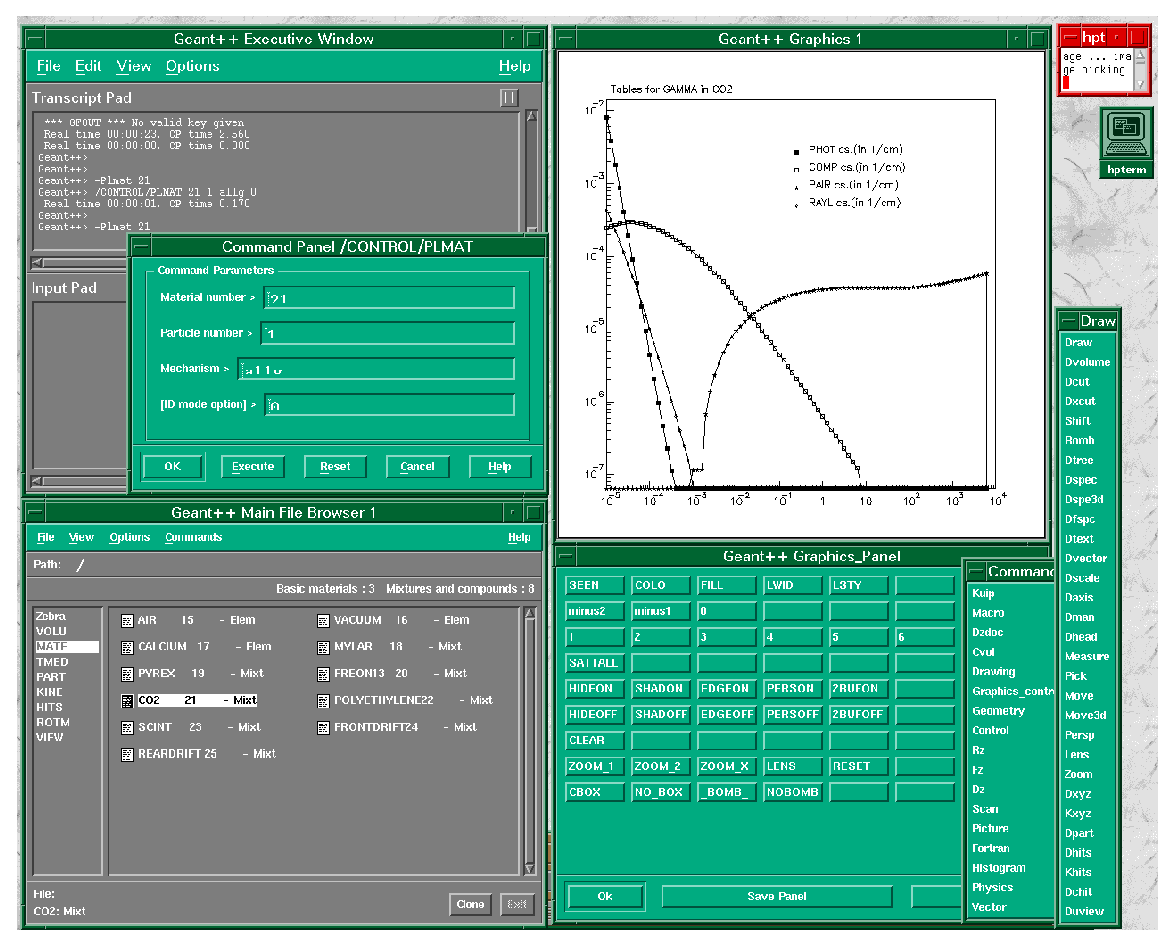
\epsfig{file=eps/motif1.eps,width=\linewidth}
      \caption{Plotting cross-sections of a material}
      \label{cons199-1}
\end{figure}

\begin{figure}[hbt]
      \centering
      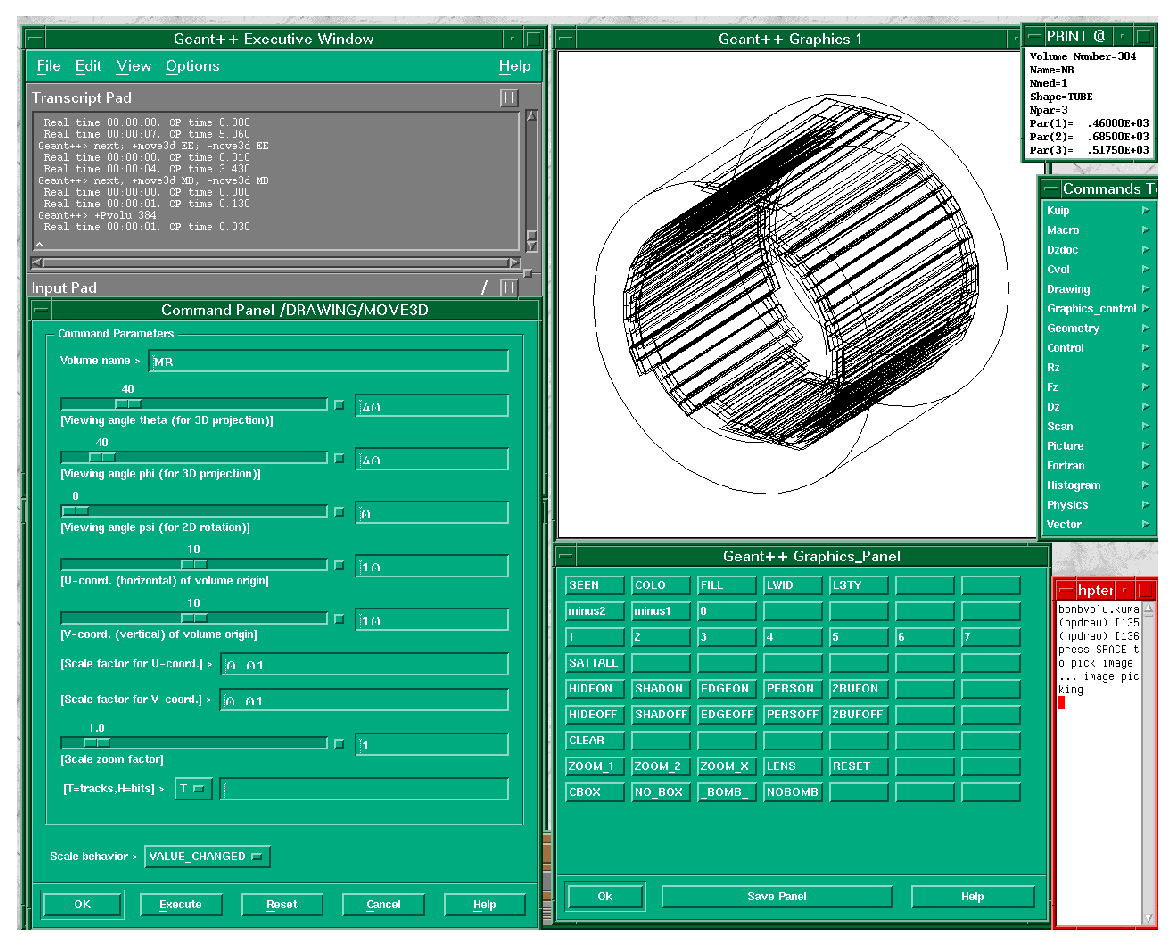
\epsfig{file=eps/motif2.eps,width=\linewidth}
      \caption{Draw using the MOVE 3D panel}
      \label{cons199-1}
\end{figure}

\putbib[cnasbibl,geabibl]
\end{bibunit}
 
%  ==================== Index material ============================

\setcounter{page}{1}%                                Reset page counter
\def\Rtnr{Index}%Dummy routine name to appear at bottom of page
\input{\jobname.ind} % index

\end{document}
